% Бүлэг 3

\pagecolor{ChapterYellow}
\chapter{Зохиомж} % 3р бүлгийн нэр
\label{Chapter3} % Энэ бүлэг рүү ишлэл хийх бол \ref{Chapter2} командыг ашигла 

%-------------------------------------------------------------------------------
%	SECTION 1
%-------------------------------------------------------------------------------

\pagecolor{white}
\section{Өгөгдлийн ерөнхий схем}

\begin{figure}[H]
    \centering
    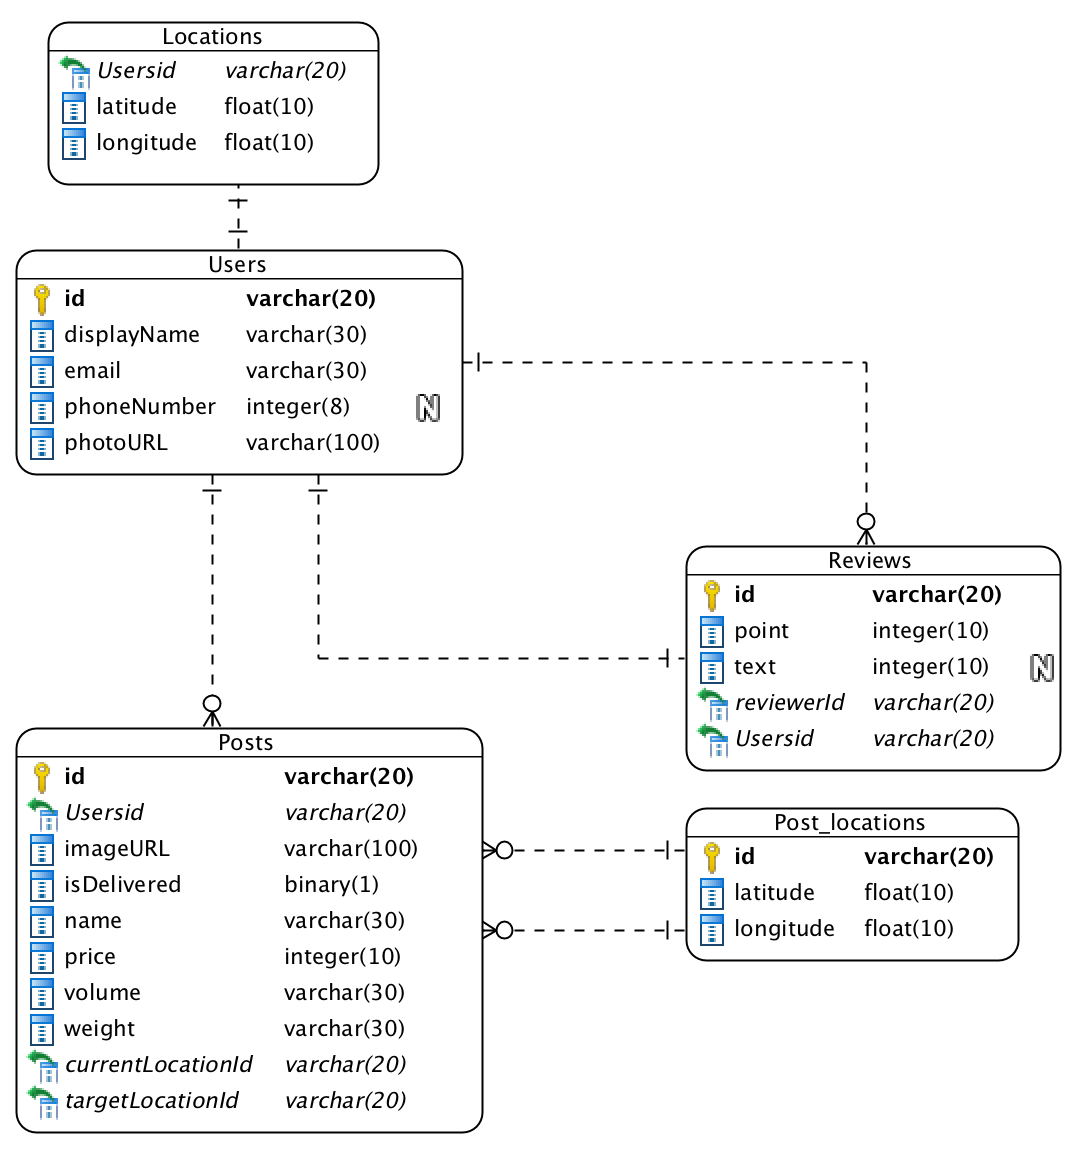
\includegraphics[width=\textwidth]{Figures/zohiomj/erd.png}
    \captionof{figure}{Өгөгдлийн ерөннхий схем}
\end{figure}

\section{Класс диаграм}

\begin{figure}[H]
    \centering
	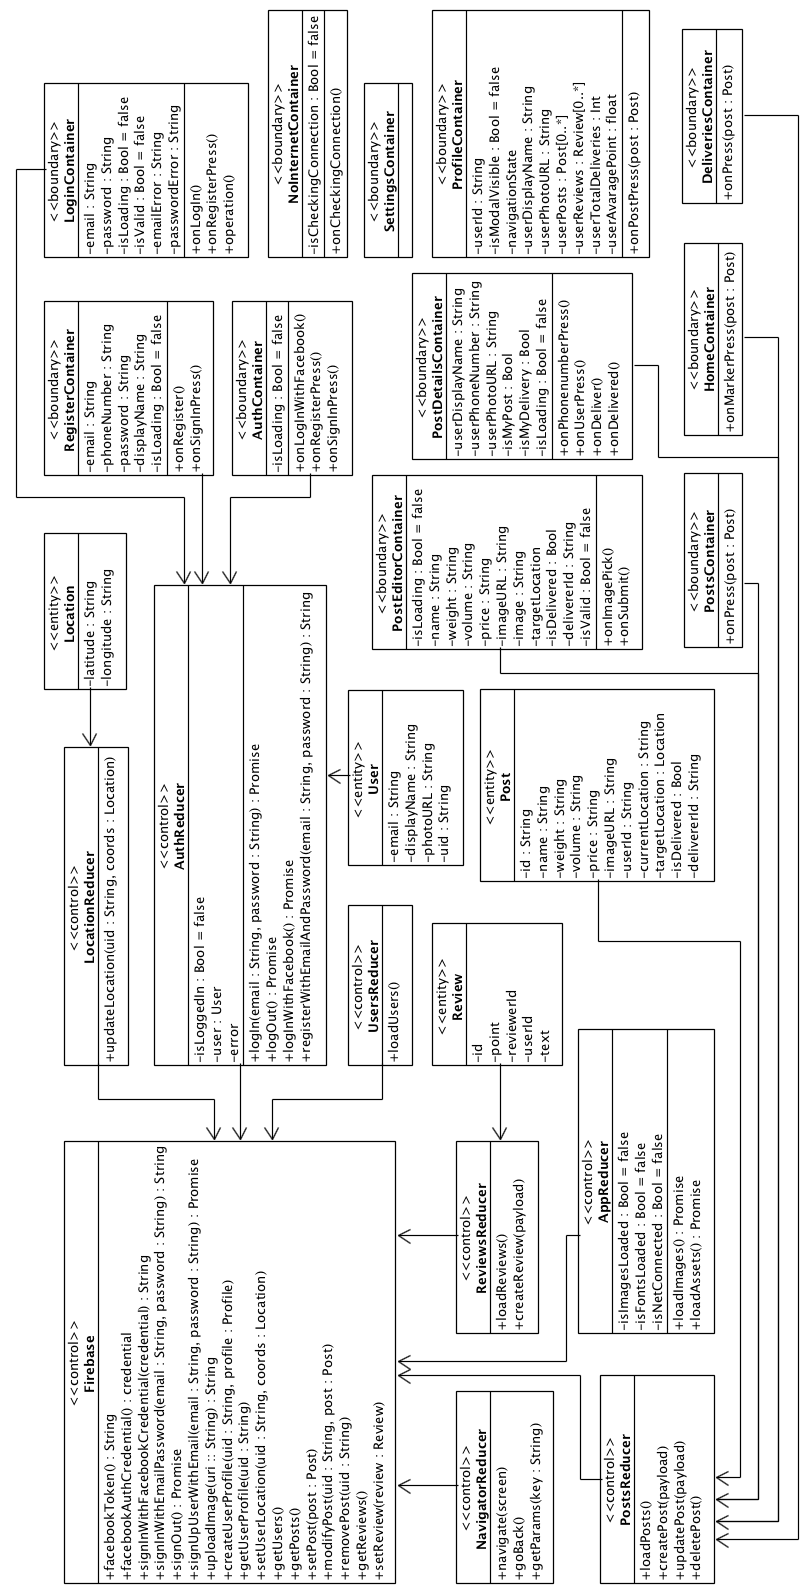
\includegraphics[height=.88\textheight]{Figures/zohiomj/upgraded_class.png}
    \captionof{figure}{Класс диаграм}
\end{figure}

% \begin{landscape} % Хуудсыг эргүүлэх

\section{Дарааллын диаграм}

\begin{figure}[H]
	\centering
	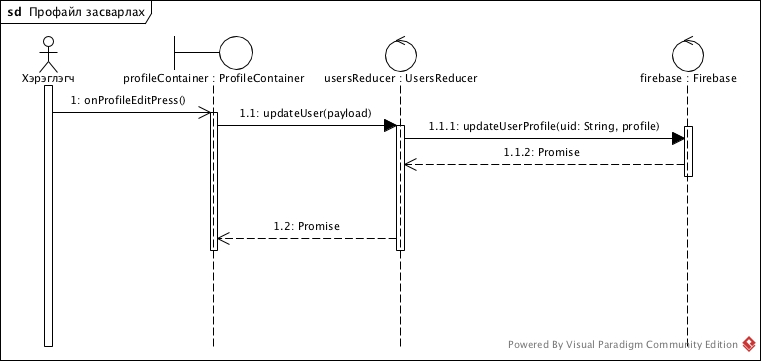
\includegraphics[width=\textwidth]{Figures/zohiomj/seq/profile_zasvarlah.jpg}
	\caption{Профайл засварлах дарааллын диаграм}
\end{figure}

\begin{figure}[H]
	\centering
	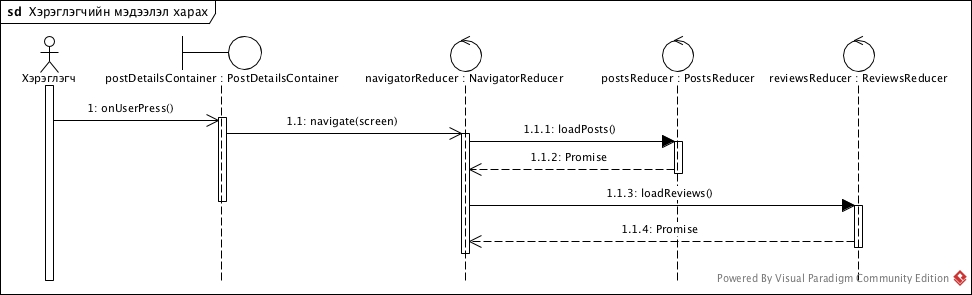
\includegraphics[width=\textwidth]{Figures/zohiomj/seq/hereglegchiin_medeelel_harah.jpg}
	\caption{Хэрэглэгчийн мэдээлэл харах дарааллын диаграм}
\end{figure}

\begin{figure}[H]
	\centering
	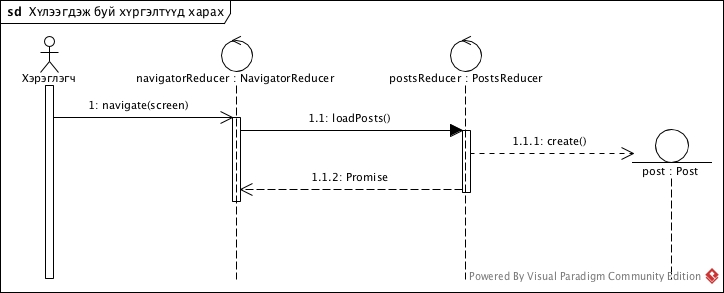
\includegraphics[width=\textwidth]{Figures/zohiomj/seq/huleegdej_bui_hurgelt_harah.jpg}
	\caption{Хүлээгдэж буй хүргэлтүүд харах дарааллын диаграм}
\end{figure}

\begin{figure}[H]
	\centering
	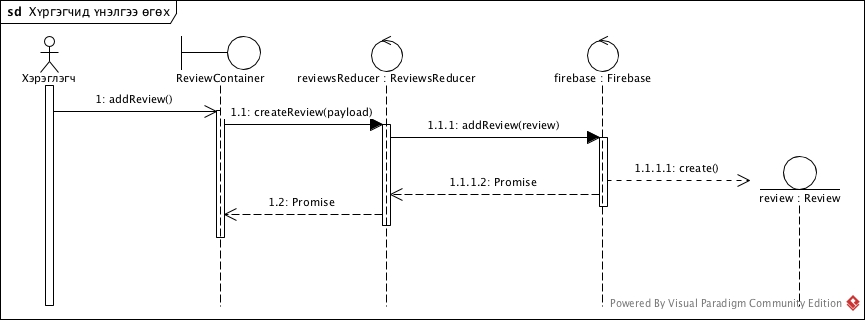
\includegraphics[width=\textwidth]{Figures/zohiomj/seq/hurgegchid_unelgee_ogoh.jpg}
	\caption{Хүргэгчид үнэлгээ өгөх дарааллын диаграм}
\end{figure}

\begin{figure}[H]
	\centering
	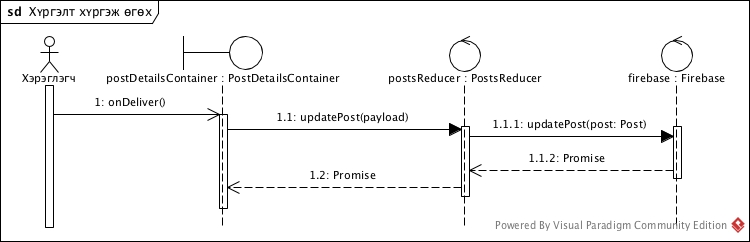
\includegraphics[width=\textwidth]{Figures/zohiomj/seq/hurgelt_hurgej_ogoh.jpg}
	\caption{Хүргэлт хүргэж өгөх дарааллын диаграм}
\end{figure}

\begin{figure}[H]
	\centering
	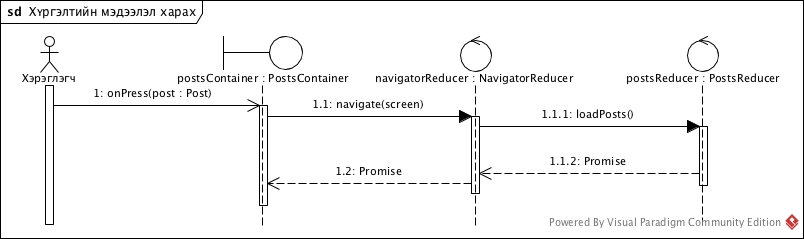
\includegraphics[width=\textwidth]{Figures/zohiomj/seq/hurgeltiin_medeelel_harah.jpg}
	\caption{Хүргэлтийн мэдээлэл харах дарааллын диаграм}
\end{figure}

\begin{figure}[H]
	\centering
	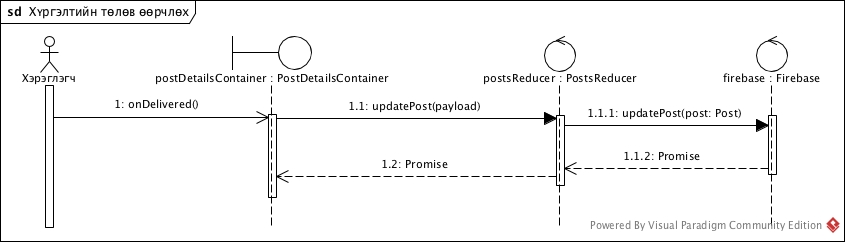
\includegraphics[width=\textwidth]{Figures/zohiomj/seq/hurgeltiin_tolov_oorchloh.jpg}
	\caption{Хүргэлтийн төлөв өөрчлөх дарааллын диаграм}
\end{figure}

\begin{figure}[H]
	\centering
	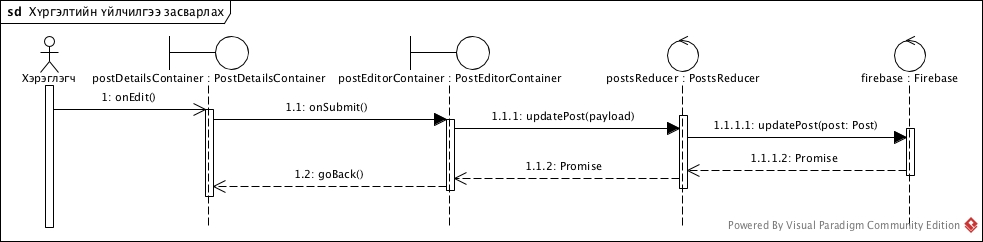
\includegraphics[width=\textwidth]{Figures/zohiomj/seq/hurgeltiin_uilchilgee_zasvarlah.jpg}
	\caption{Хүргэлтийн үйлчилгээ засварлах дарааллын диаграм}
\end{figure}

\begin{figure}[H]
	\centering
	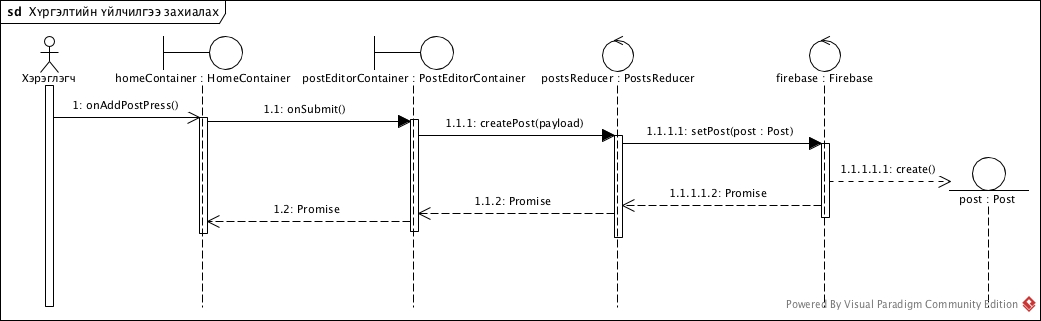
\includegraphics[width=\textwidth]{Figures/zohiomj/seq/hurgeltiin_uilchilgee_zahialah.jpg}
	\caption{Хүргэлтийн үйлчилгээ захиалах дарааллын диаграм}
\end{figure}

\begin{figure}[H]
	\centering
	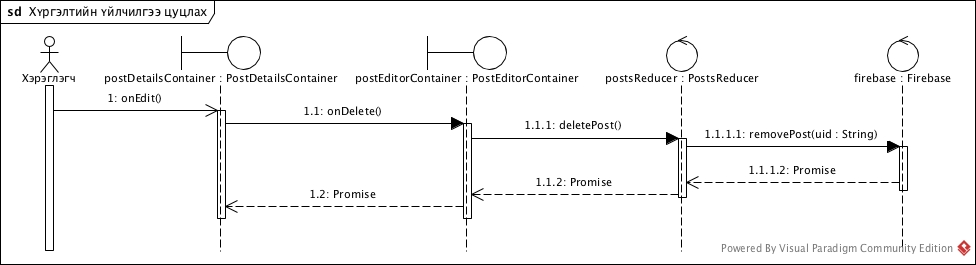
\includegraphics[width=\textwidth]{Figures/zohiomj/seq/hurgeltiin_uilchilgee_tsutslah.jpg}
	\caption{Хүргэлтийн үйлчилгээ цуцлах дарааллын диаграм}
\end{figure}

% \end{landscape}


% \begin{landscape} % Хуудсыг эргүүлэх
\section{Хэрэглэгчийн интерфейс}

\begin{figure}[H]
	\centering
    \subcaptionbox{Анхны дэлгэц}{
        
\includegraphics[height=.41\textheight, frame]{Figures/interfaces/interface1.png}
    }
    \hfill
    \subcaptionbox{Нэвтрэх дэлгэц}{
        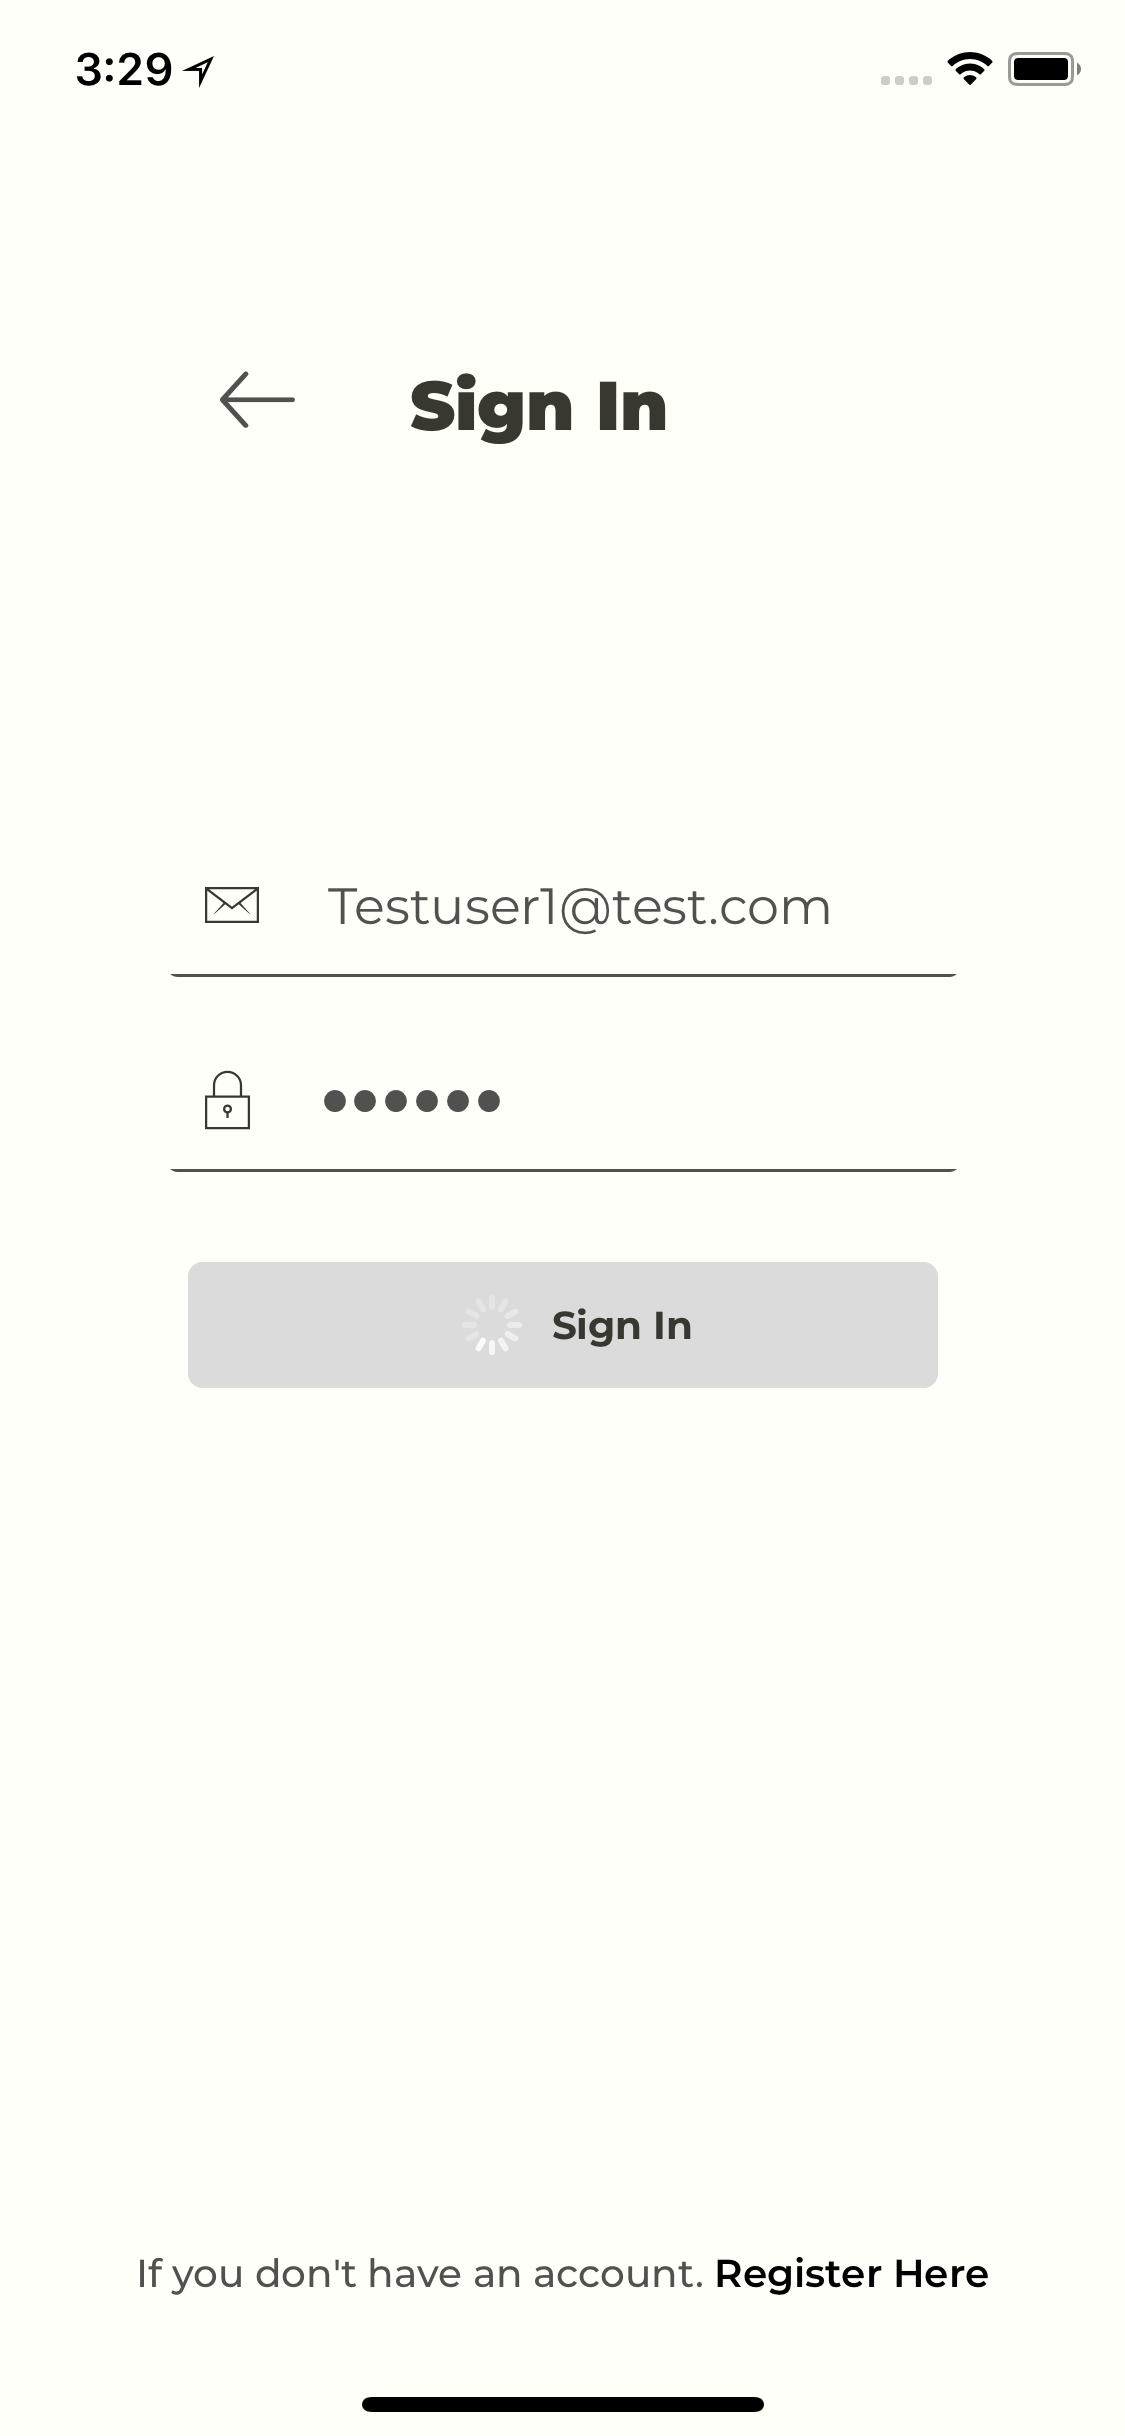
\includegraphics[height=.41\textheight, frame]{Figures/interfaces/interface2.png}
    }
    \subcaptionbox{Бүртгүүлэх дэлгэц}{
        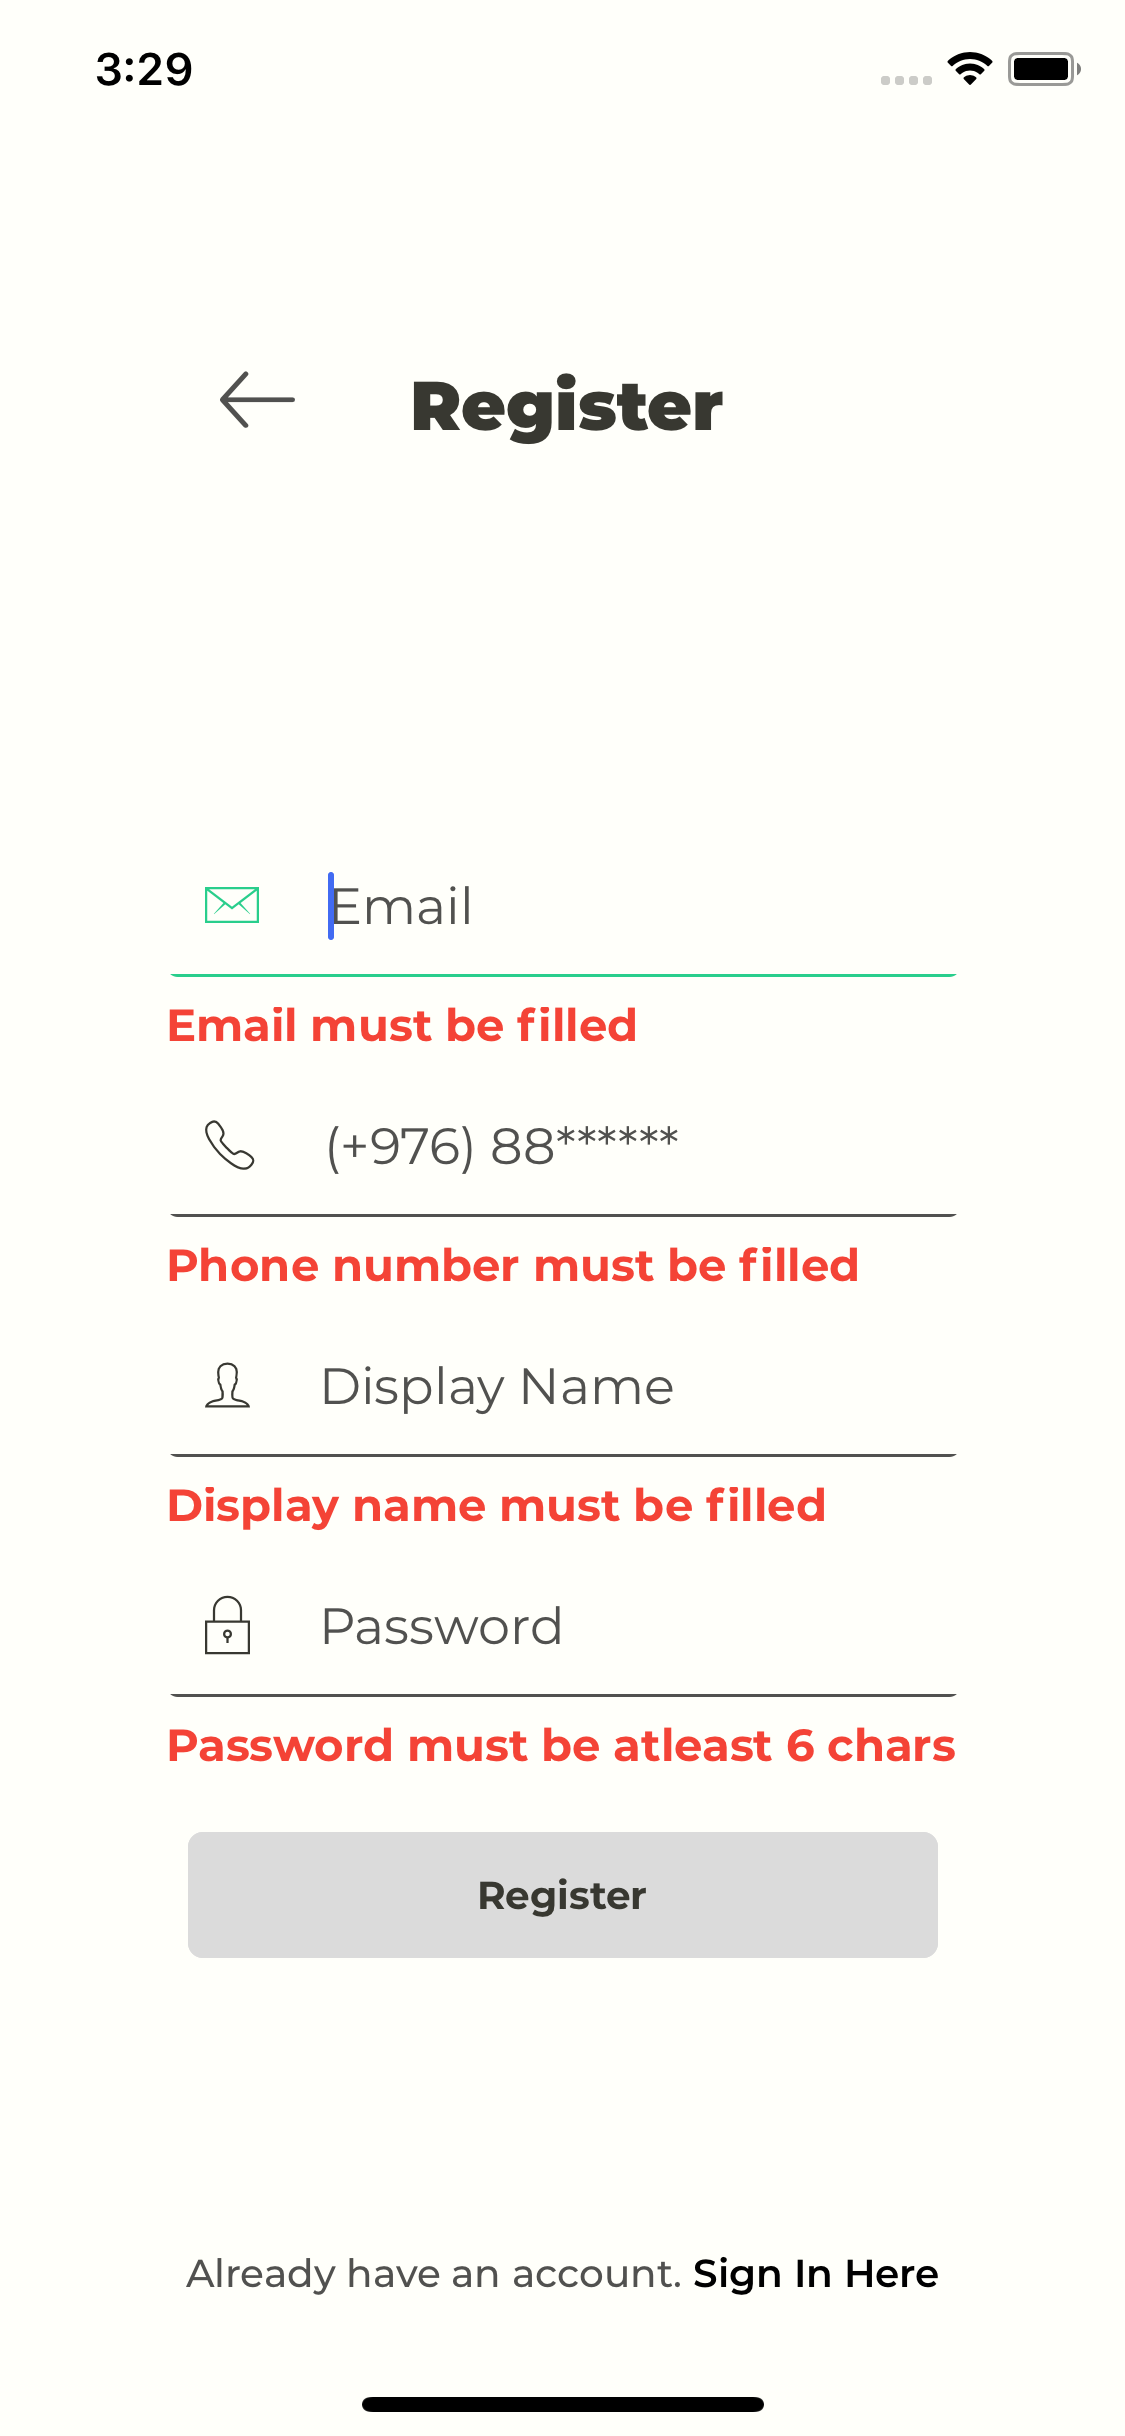
\includegraphics[height=.41\textheight, frame]{Figures/interfaces/interface3.png}
    }
    \hfill
    \subcaptionbox{Facebook нэвтрэх}{
        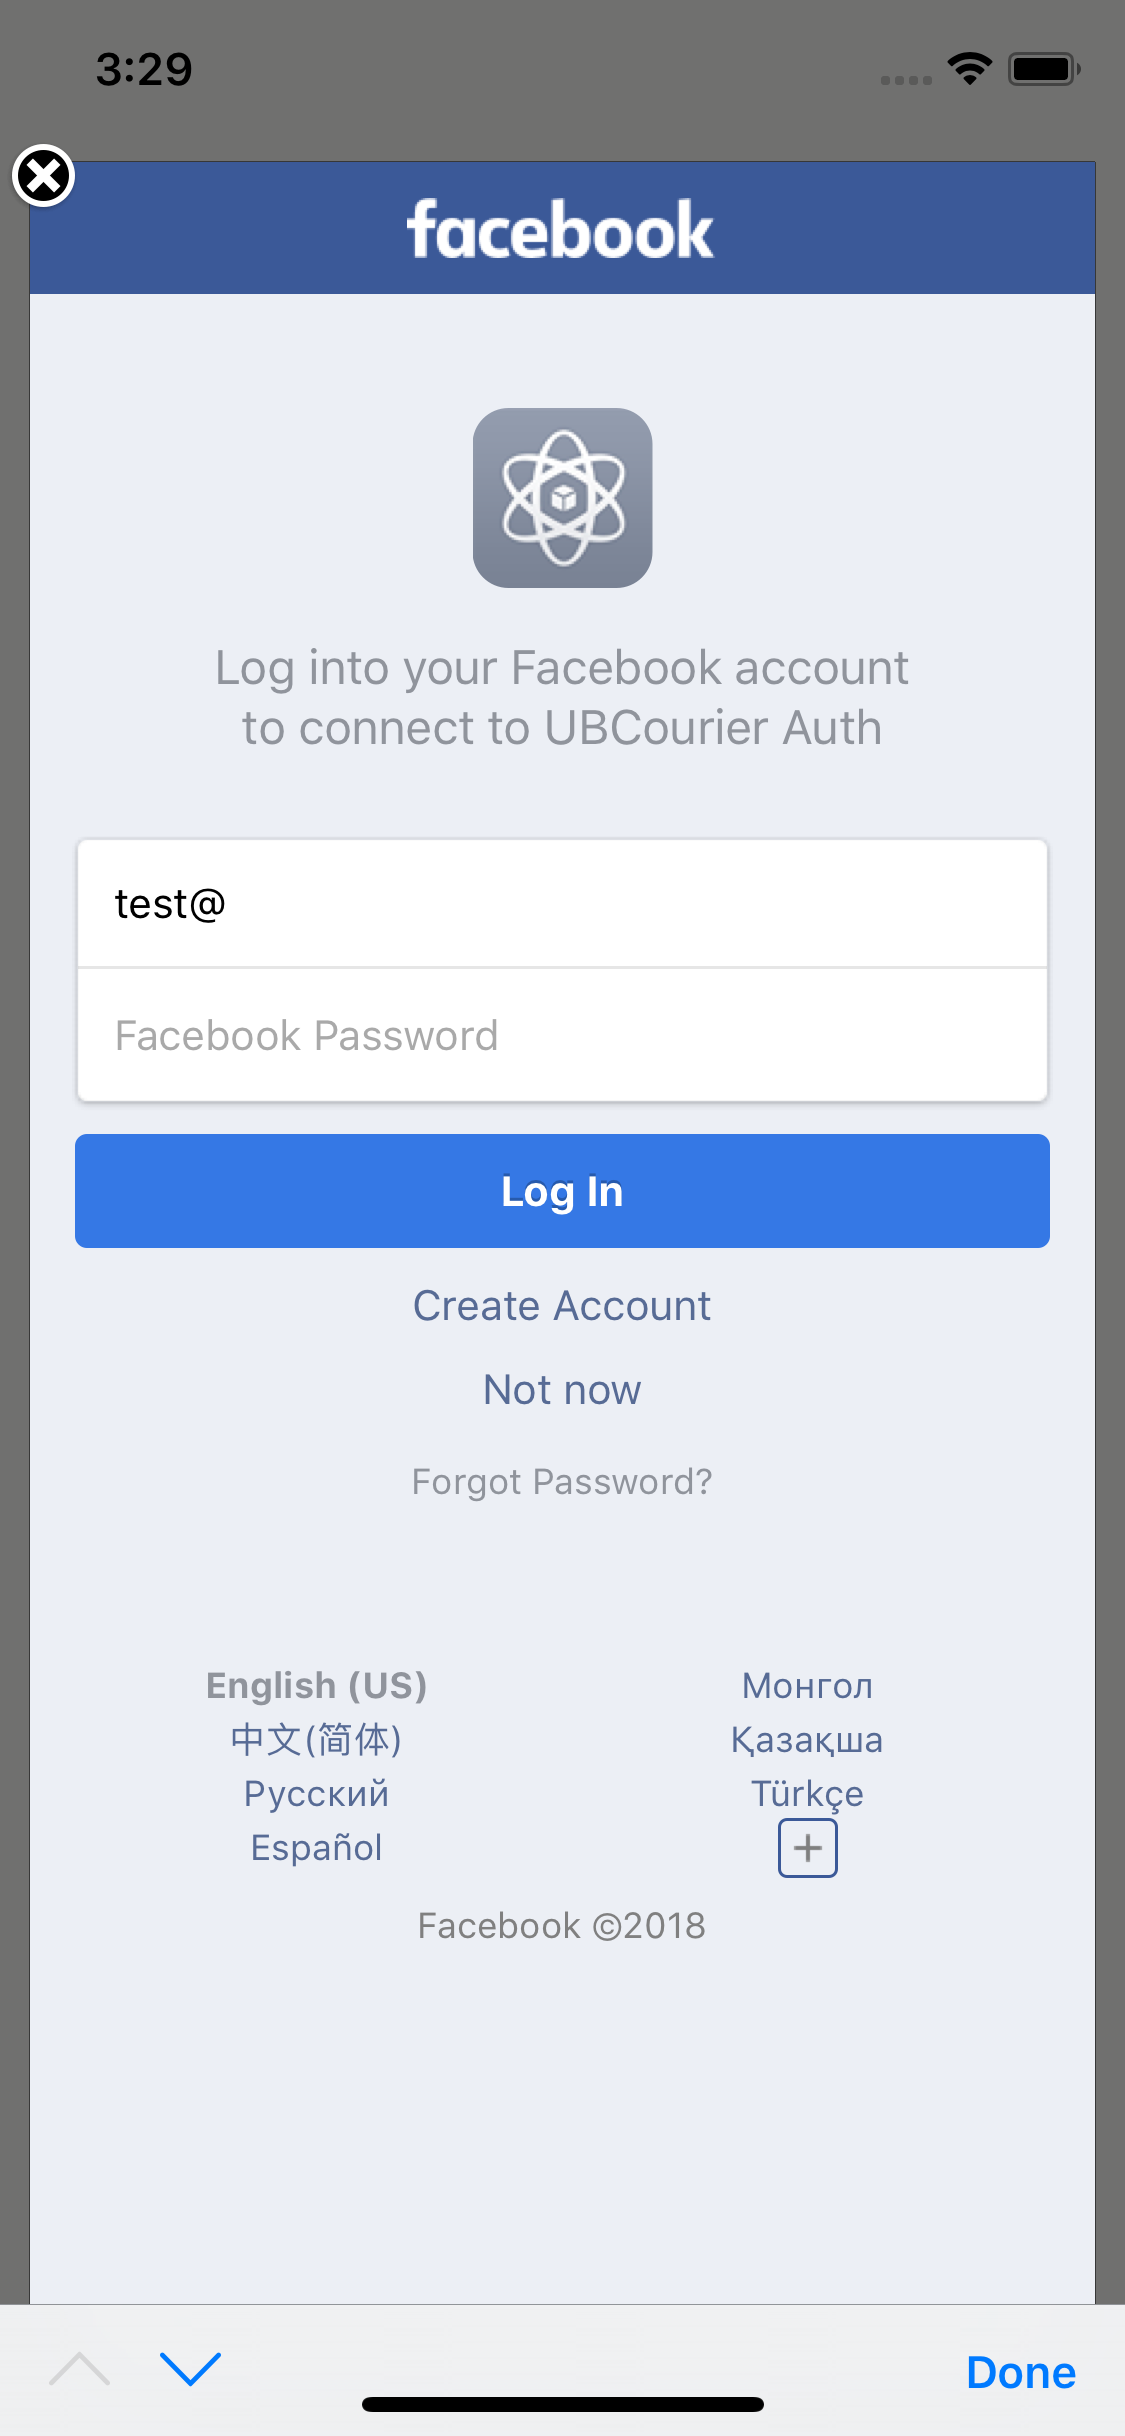
\includegraphics[height=.41\textheight, frame]{Figures/interfaces/interface4.png}
    }
    \hfill
	\caption{Нэвтрэх болон бүртгүүлэх дэлгэцийн интерфейс}
\end{figure}

\begin{figure}[H]
	\centering
    \subcaptionbox{Нэвтэрсний дараах дэлгэц}{
        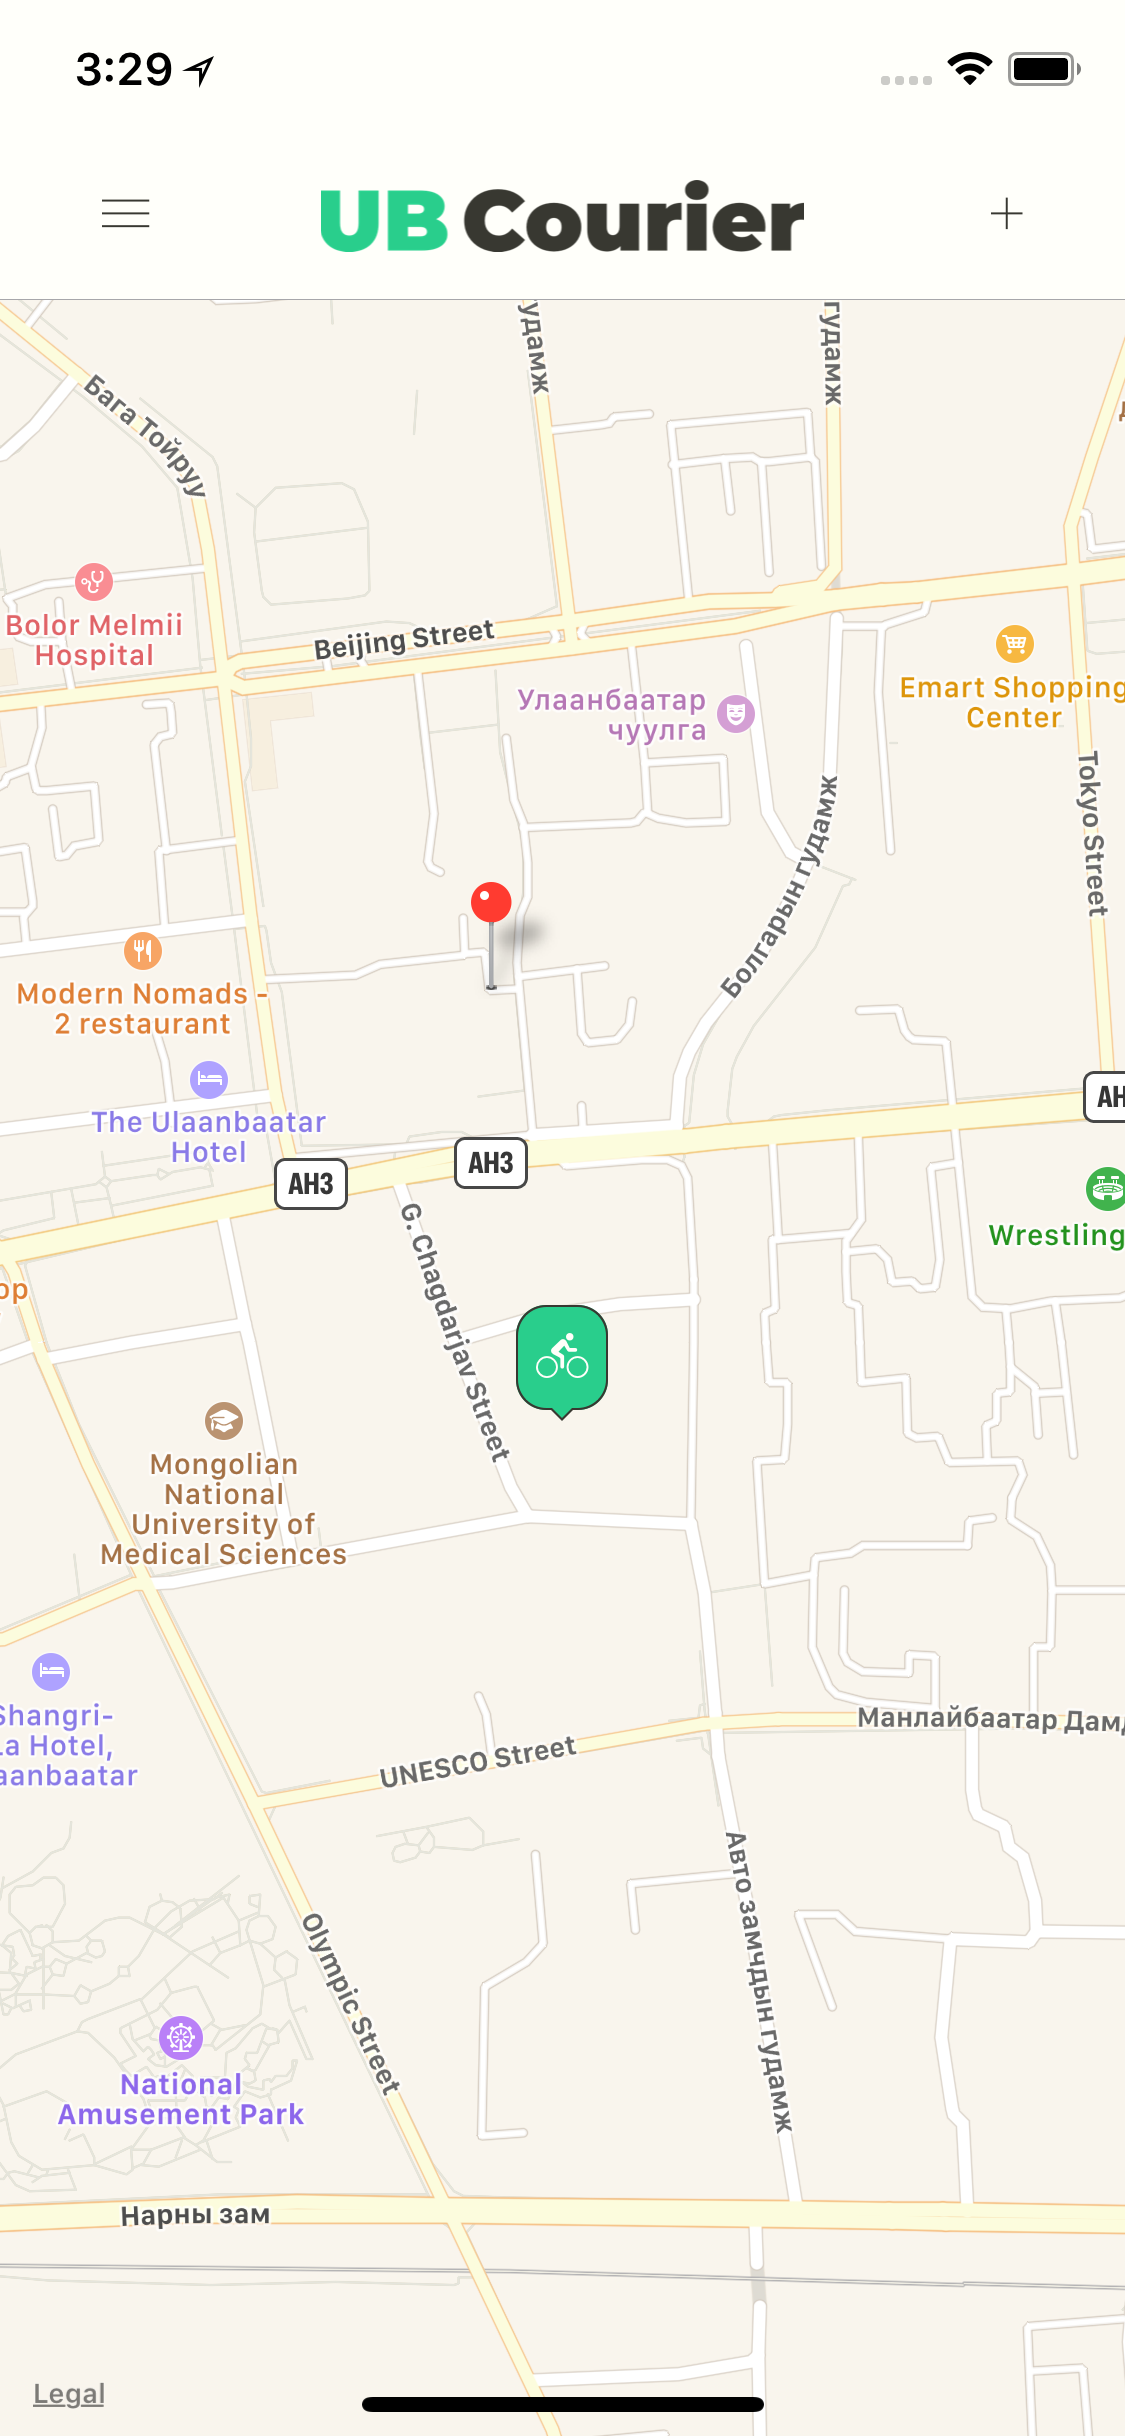
\includegraphics[width=.45\textwidth, frame]{Figures/interfaces/interface5.png}
    }
    \hfill
    \subcaptionbox{Цэсийн дэлгэсэн байдал}{
        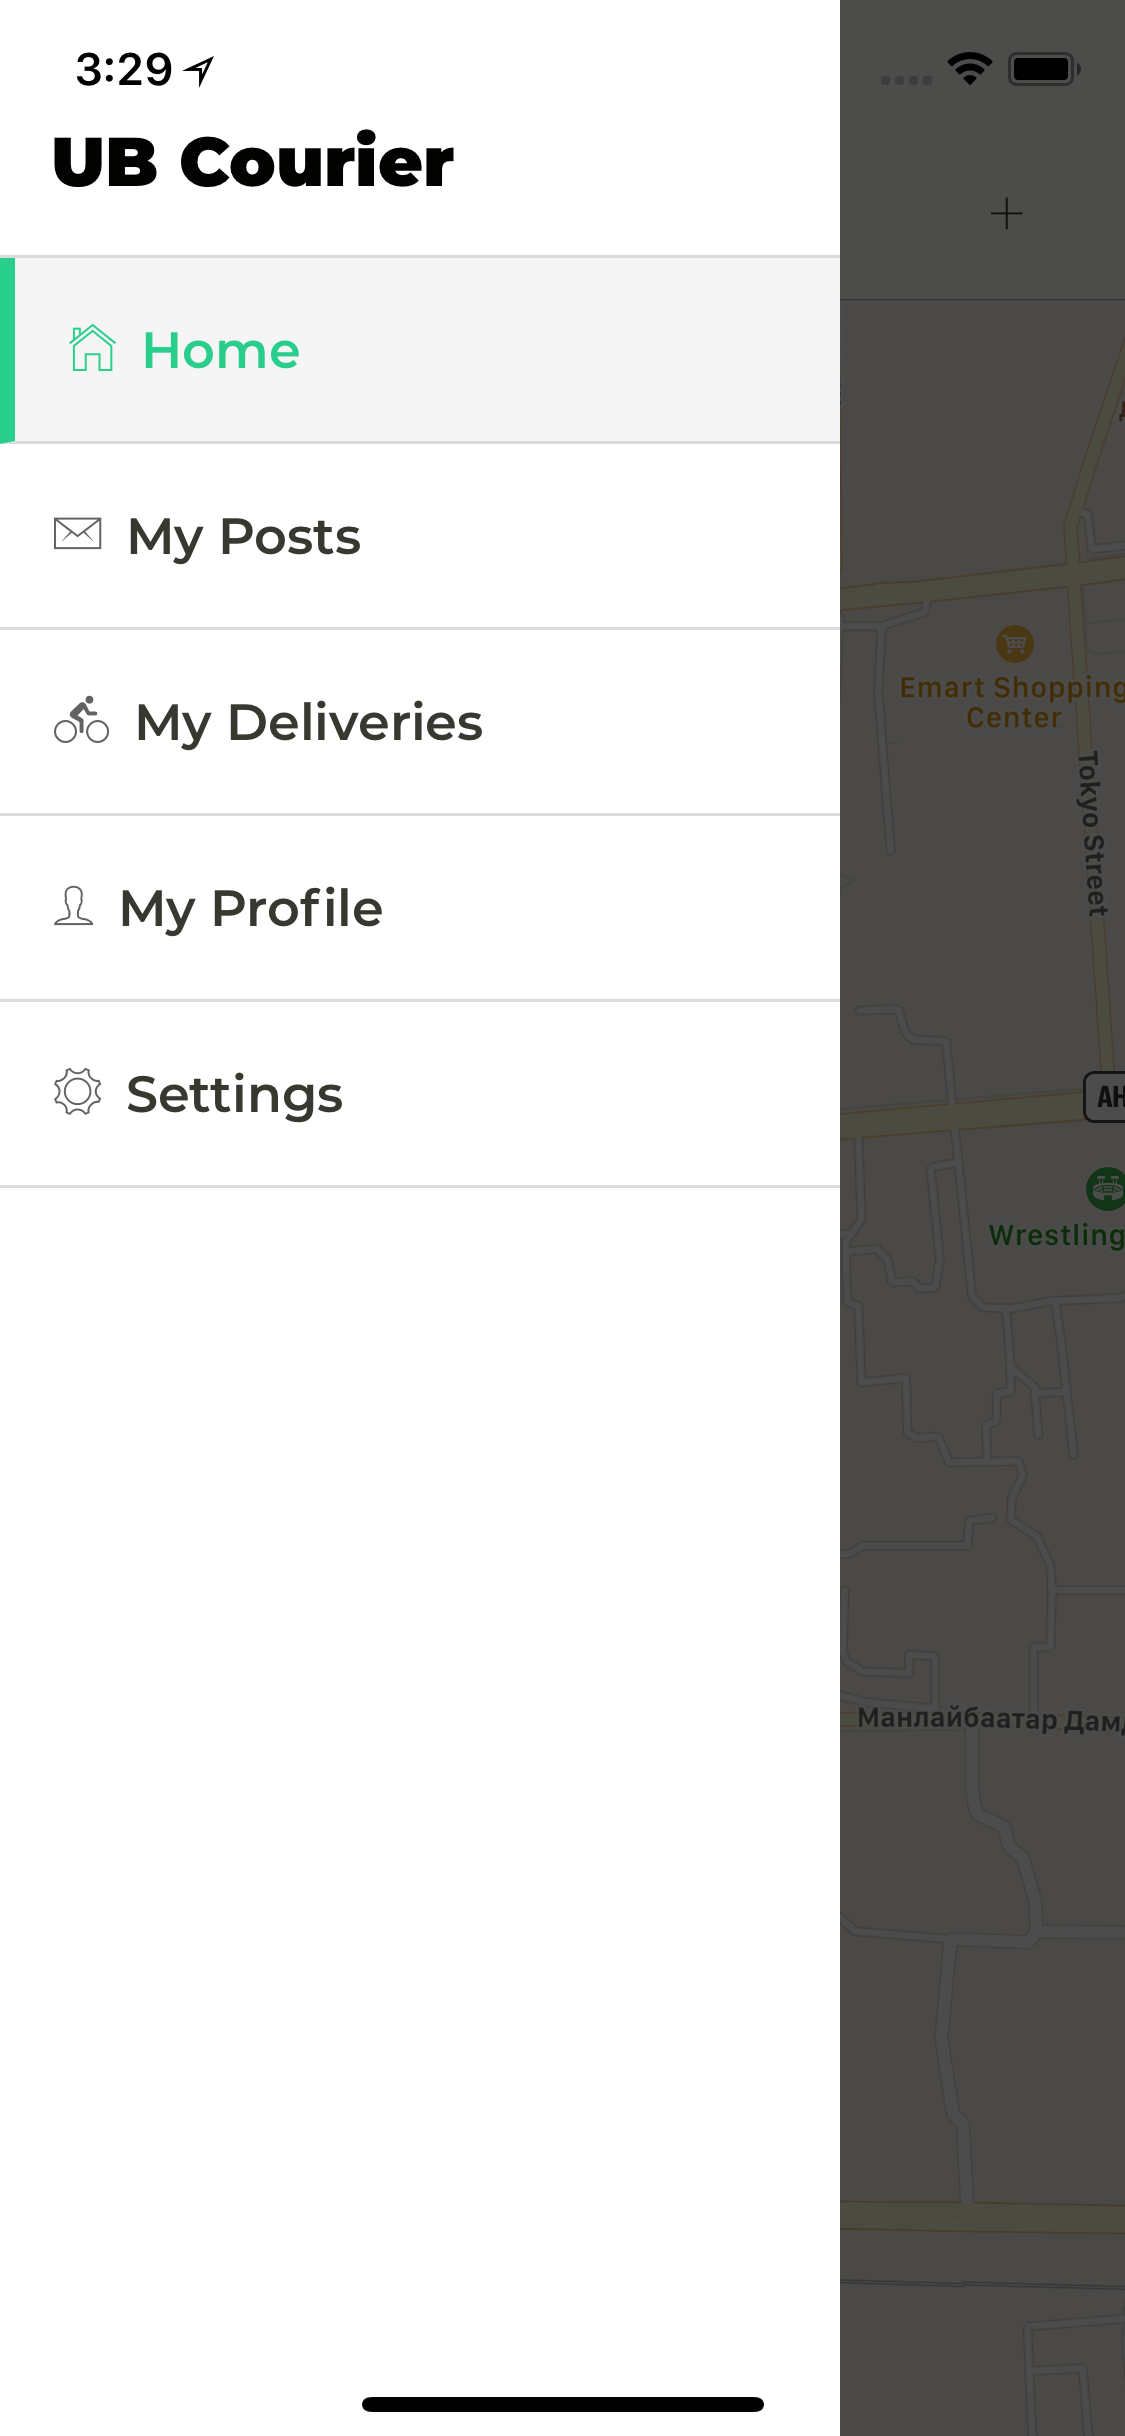
\includegraphics[width=.45\textwidth, frame]{Figures/interfaces/interface6.png}
    }
	\caption{Үндсэн дэлгэц болон цэсний интерфейс}
\end{figure}

\begin{figure}[H]
	\centering
    \subcaptionbox{Миний хүргэлтийн захиалгууд}{
        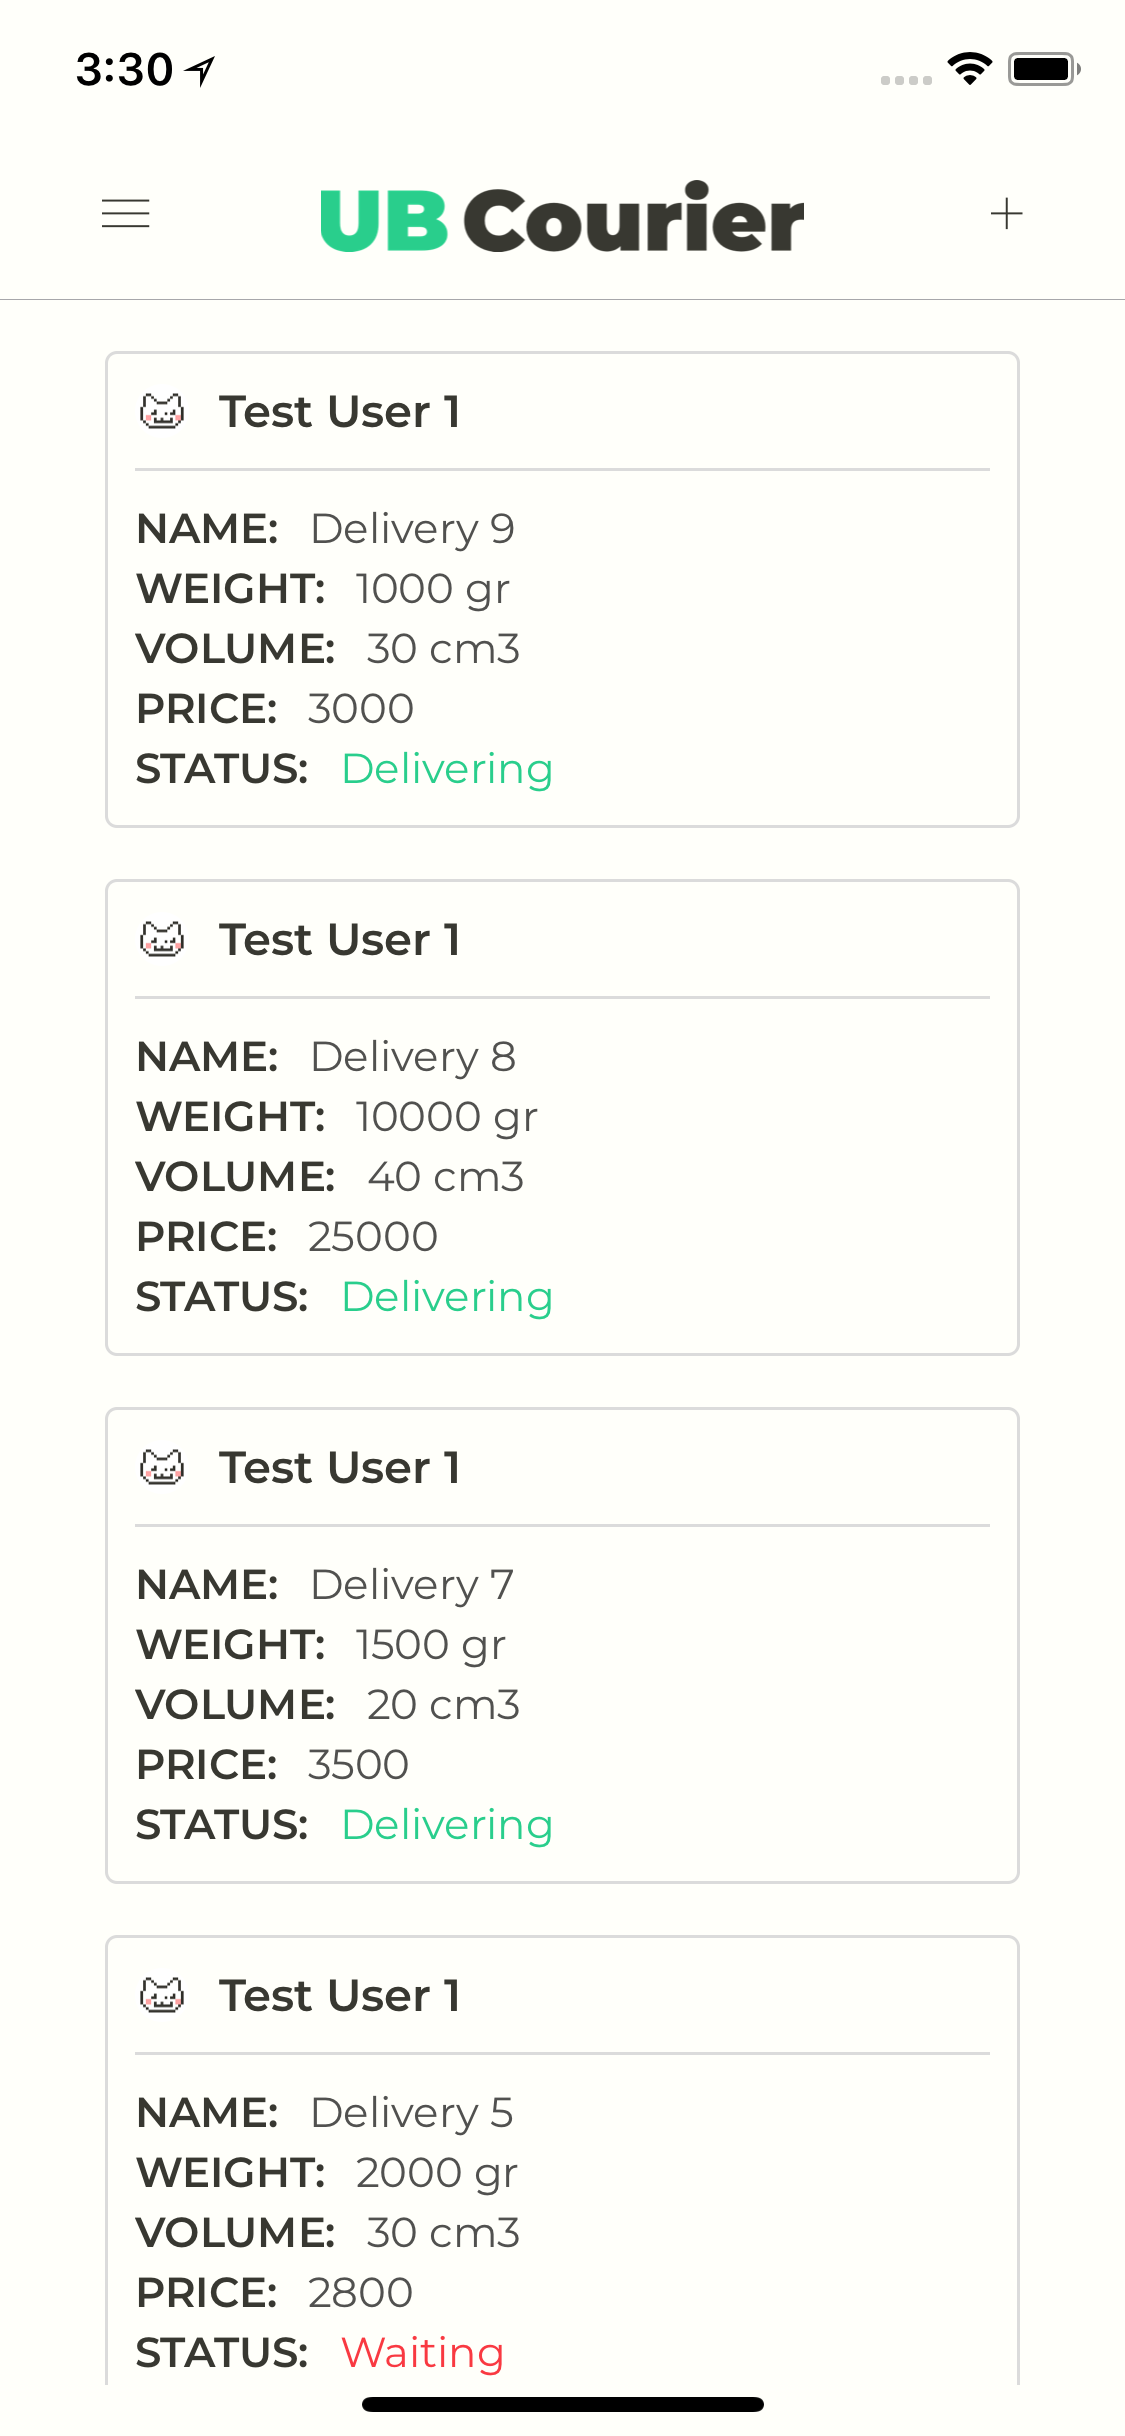
\includegraphics[width=.3\textwidth, frame]{Figures/interfaces/interface7.png}
    }
    \hfill
    \subcaptionbox{Миний хүргэлтүүд}{
        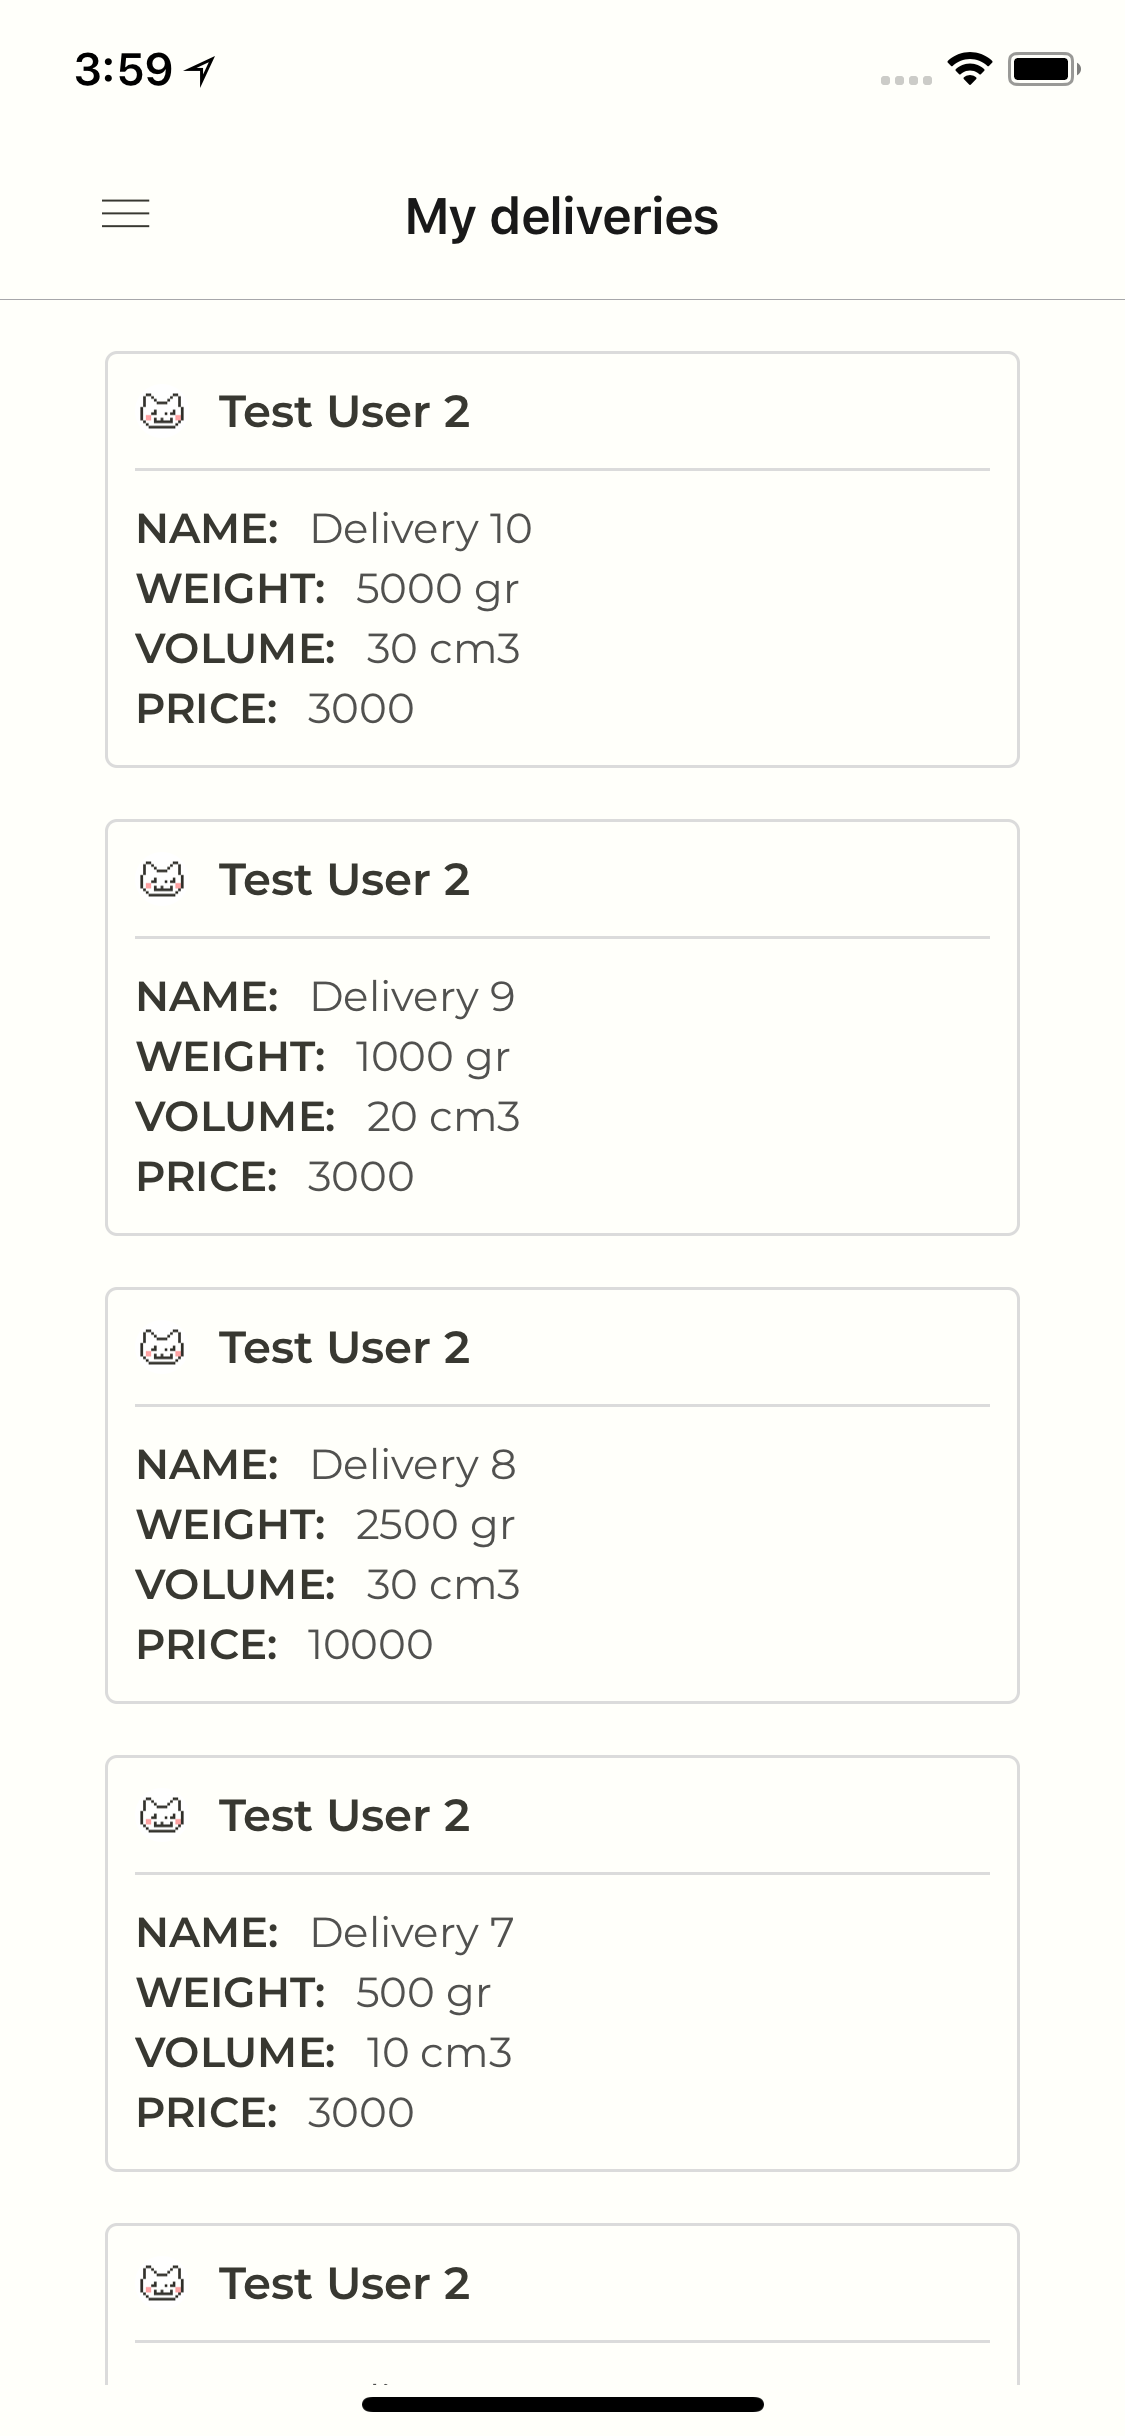
\includegraphics[width=.3\textwidth, frame]{Figures/interfaces/interface8.png}
    }
    \hfill
    \subcaptionbox{Шинэ захиалга}{
        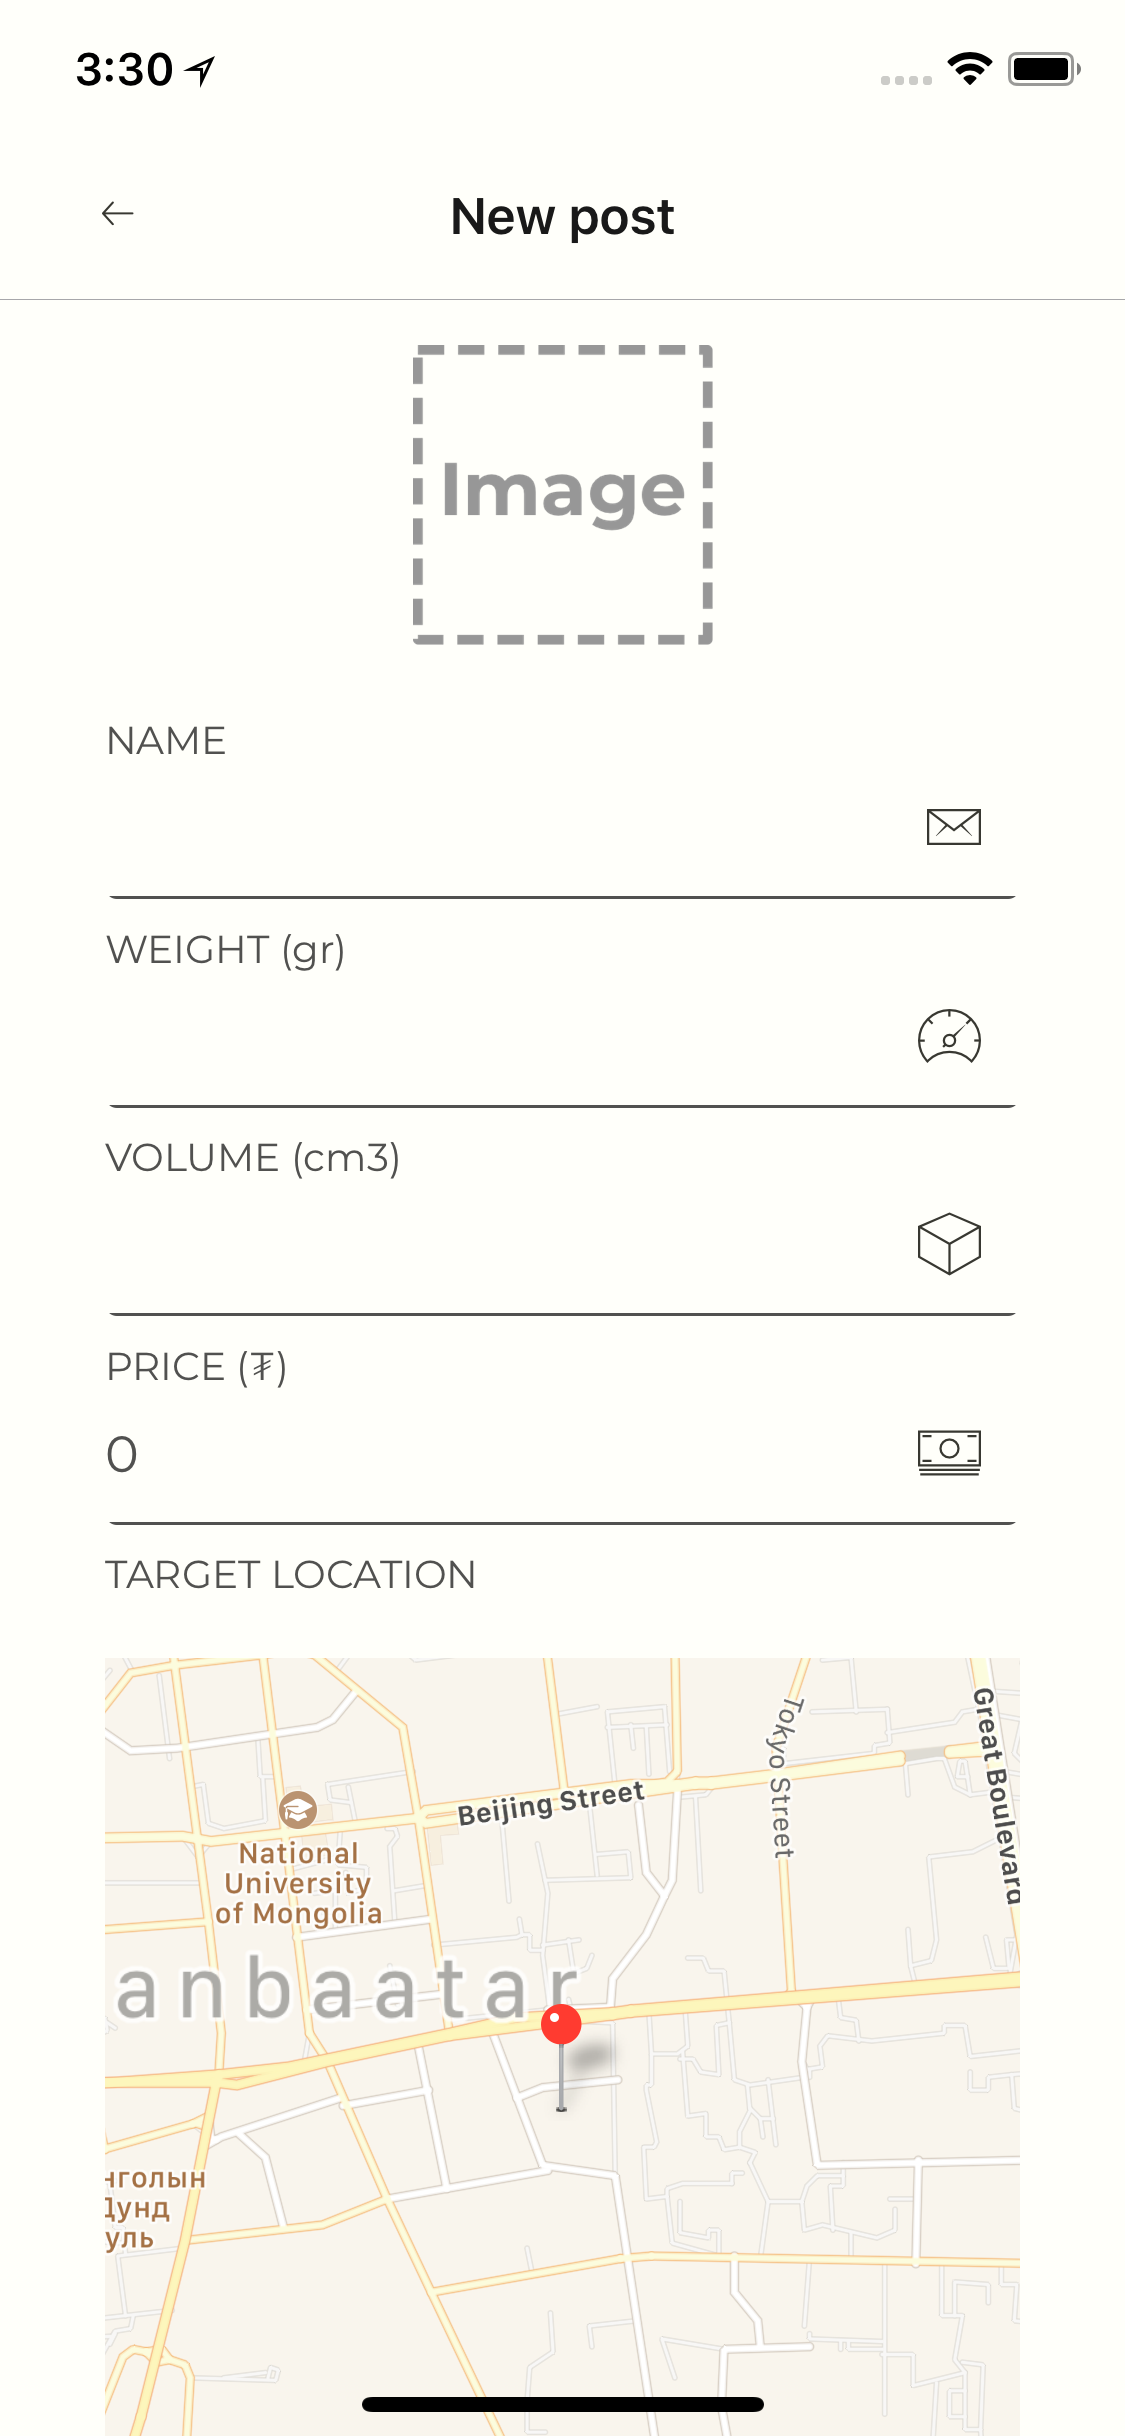
\includegraphics[width=.3\textwidth, frame]{Figures/interfaces/interface9.png}
    }
	\caption{Хүргэлтүүдийн дэлгэцийн интерфэйс}
\end{figure}

\begin{figure}[H]
	\centering
    \subcaptionbox{Миний хүргэлт}{
        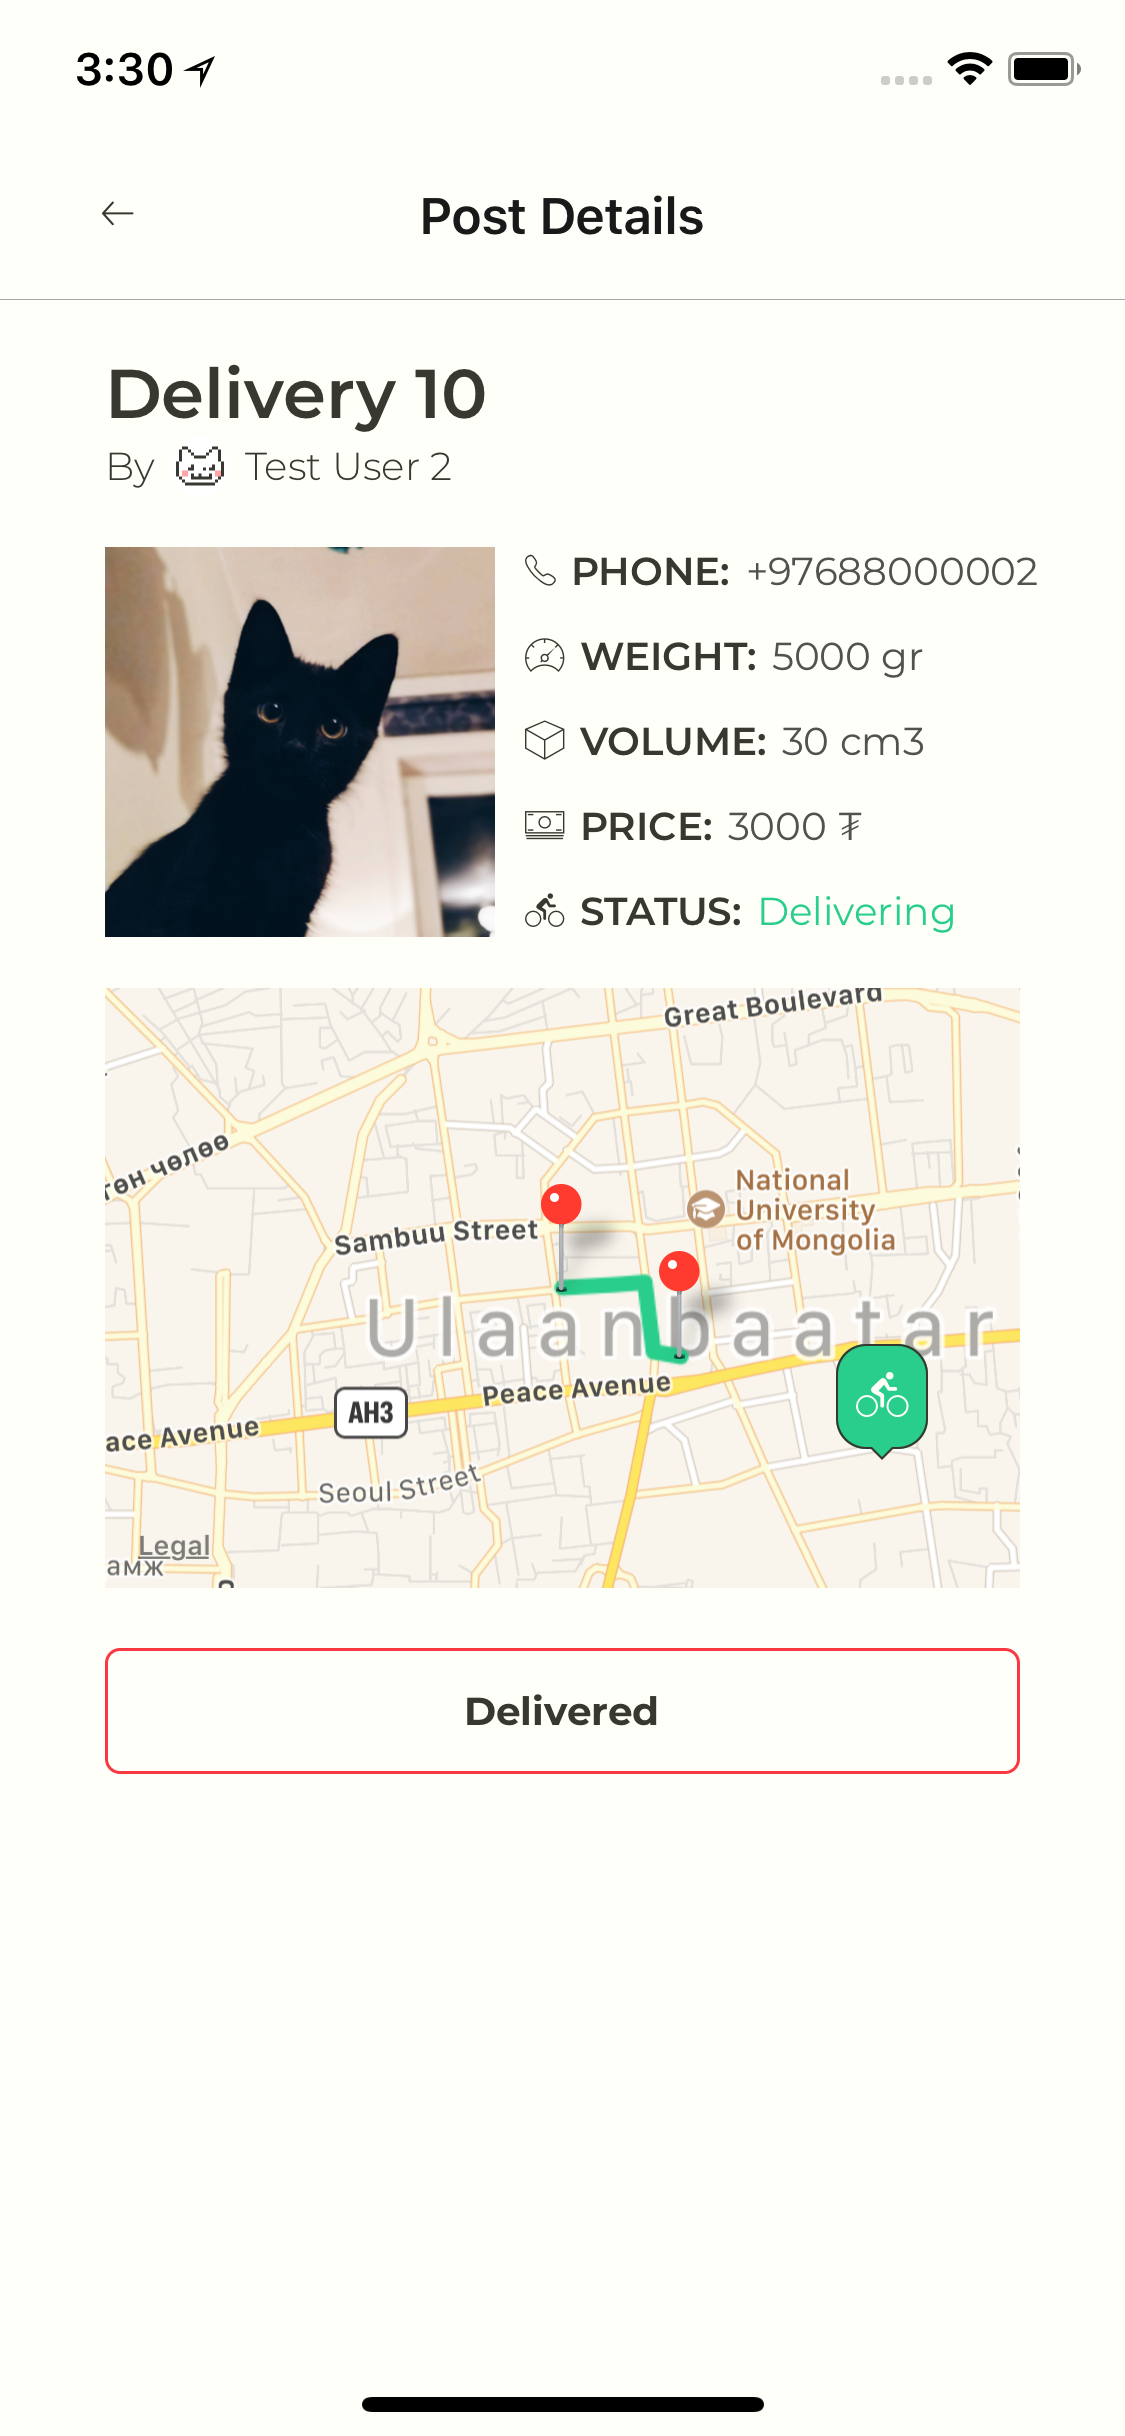
\includegraphics[width=.3\textwidth, frame]{Figures/interfaces/interface10.png}
    }
    \hfill
    \subcaptionbox{Миний хүргэлтийн захиалга}{
        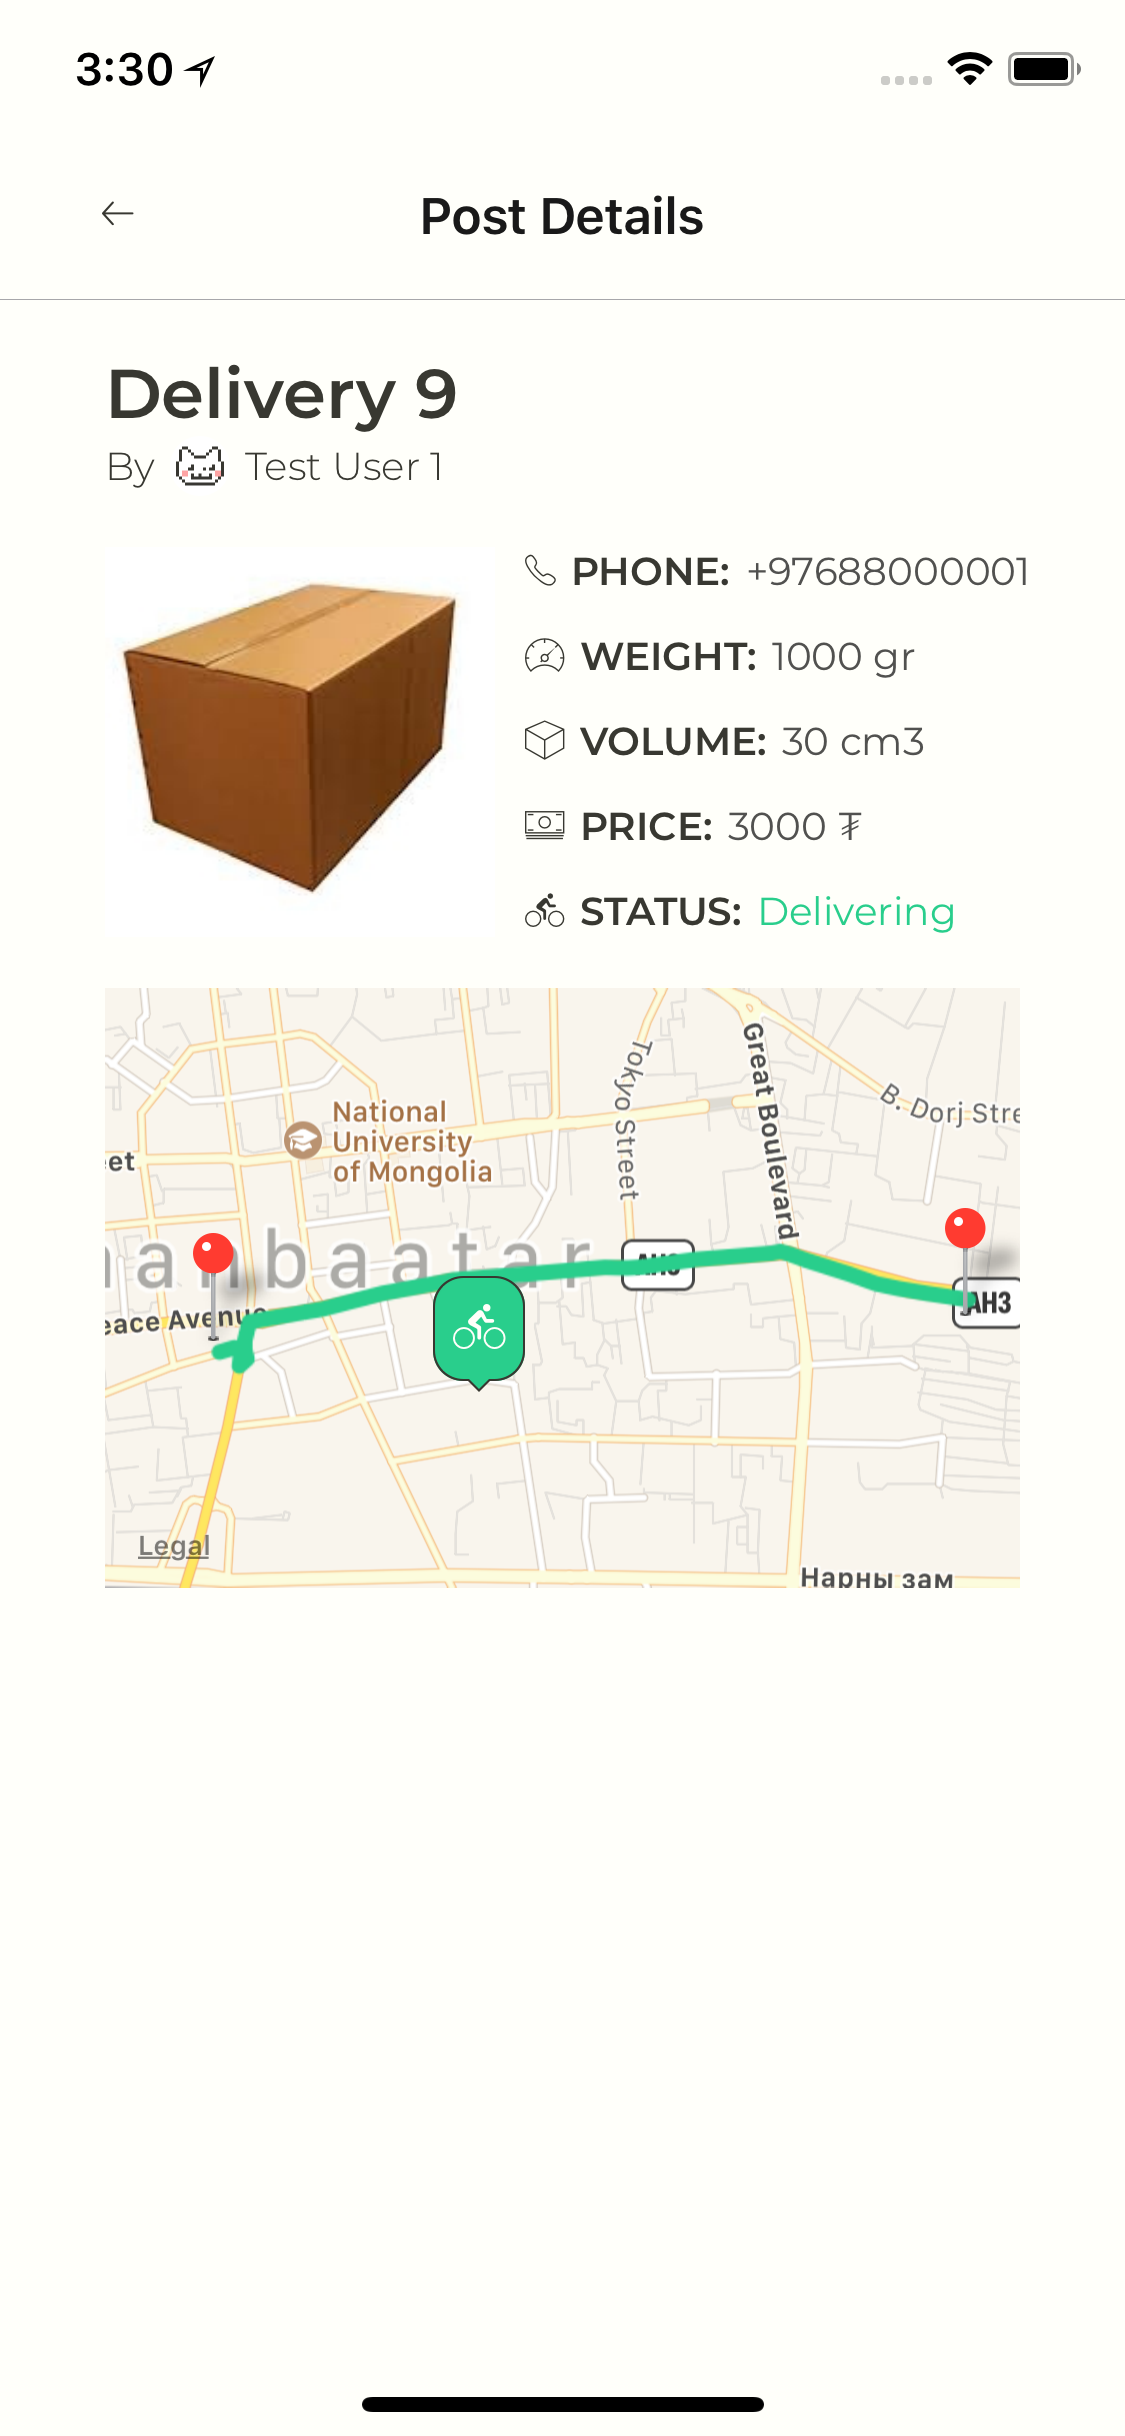
\includegraphics[width=.3\textwidth, frame]{Figures/interfaces/interface11.png}
    }
    \hfill
    \subcaptionbox{Хүргэгчгүй хүргэлт}{
        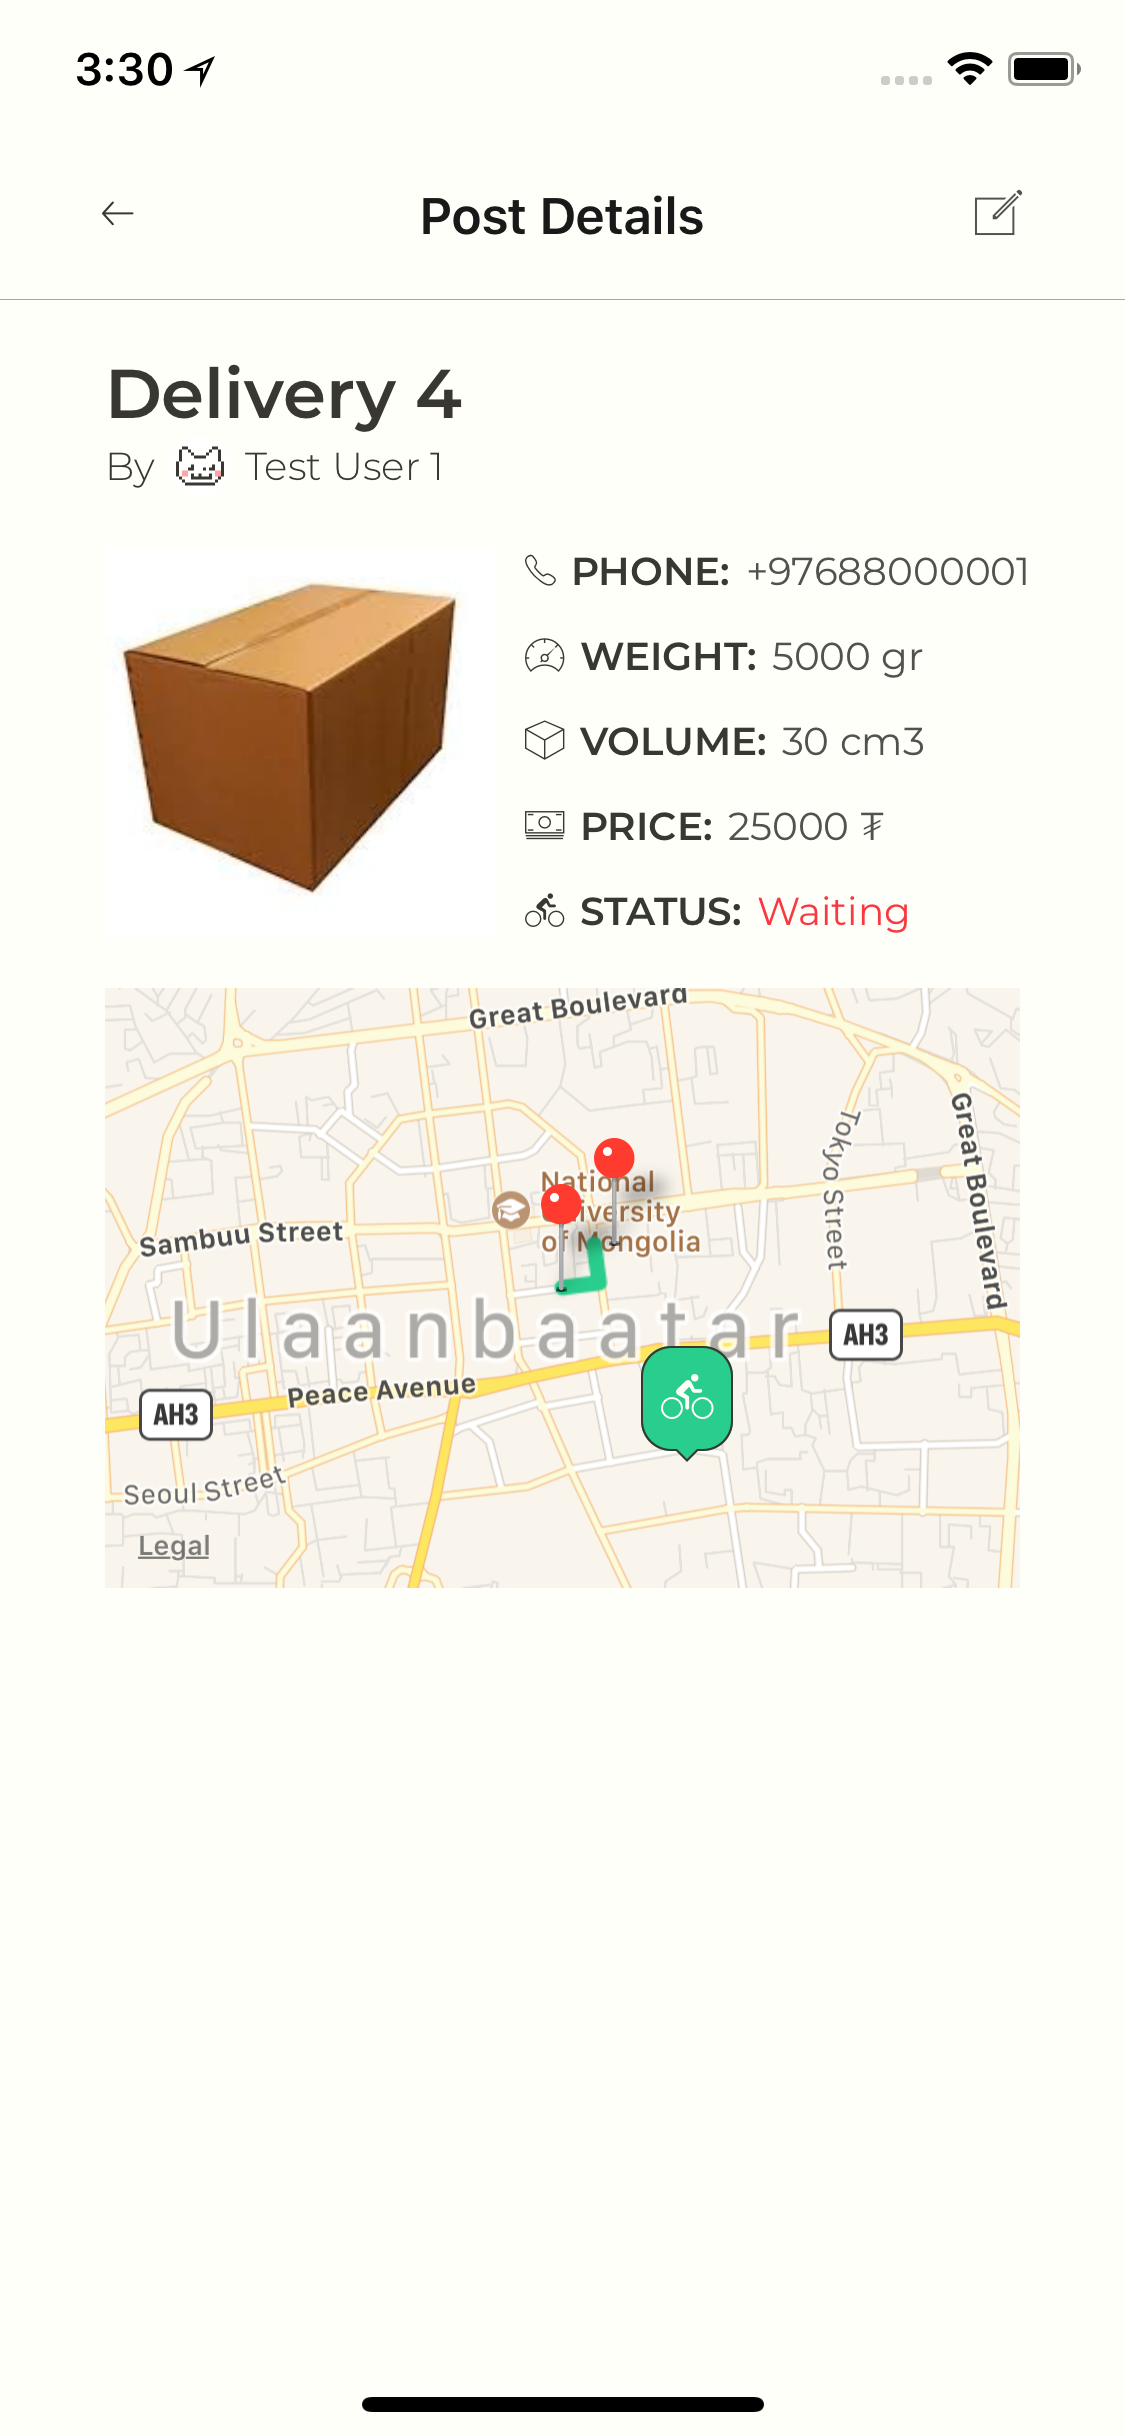
\includegraphics[width=.3\textwidth, frame]{Figures/interfaces/interface12.png}
    }
	\caption{Хүргэлтийн мэдээллүүд дэлгэцийн интерфэйс}
\end{figure}

\begin{figure}[H]
	\centering
    \subcaptionbox{Хэрэглэгчийн хүргэлтүүд}{
        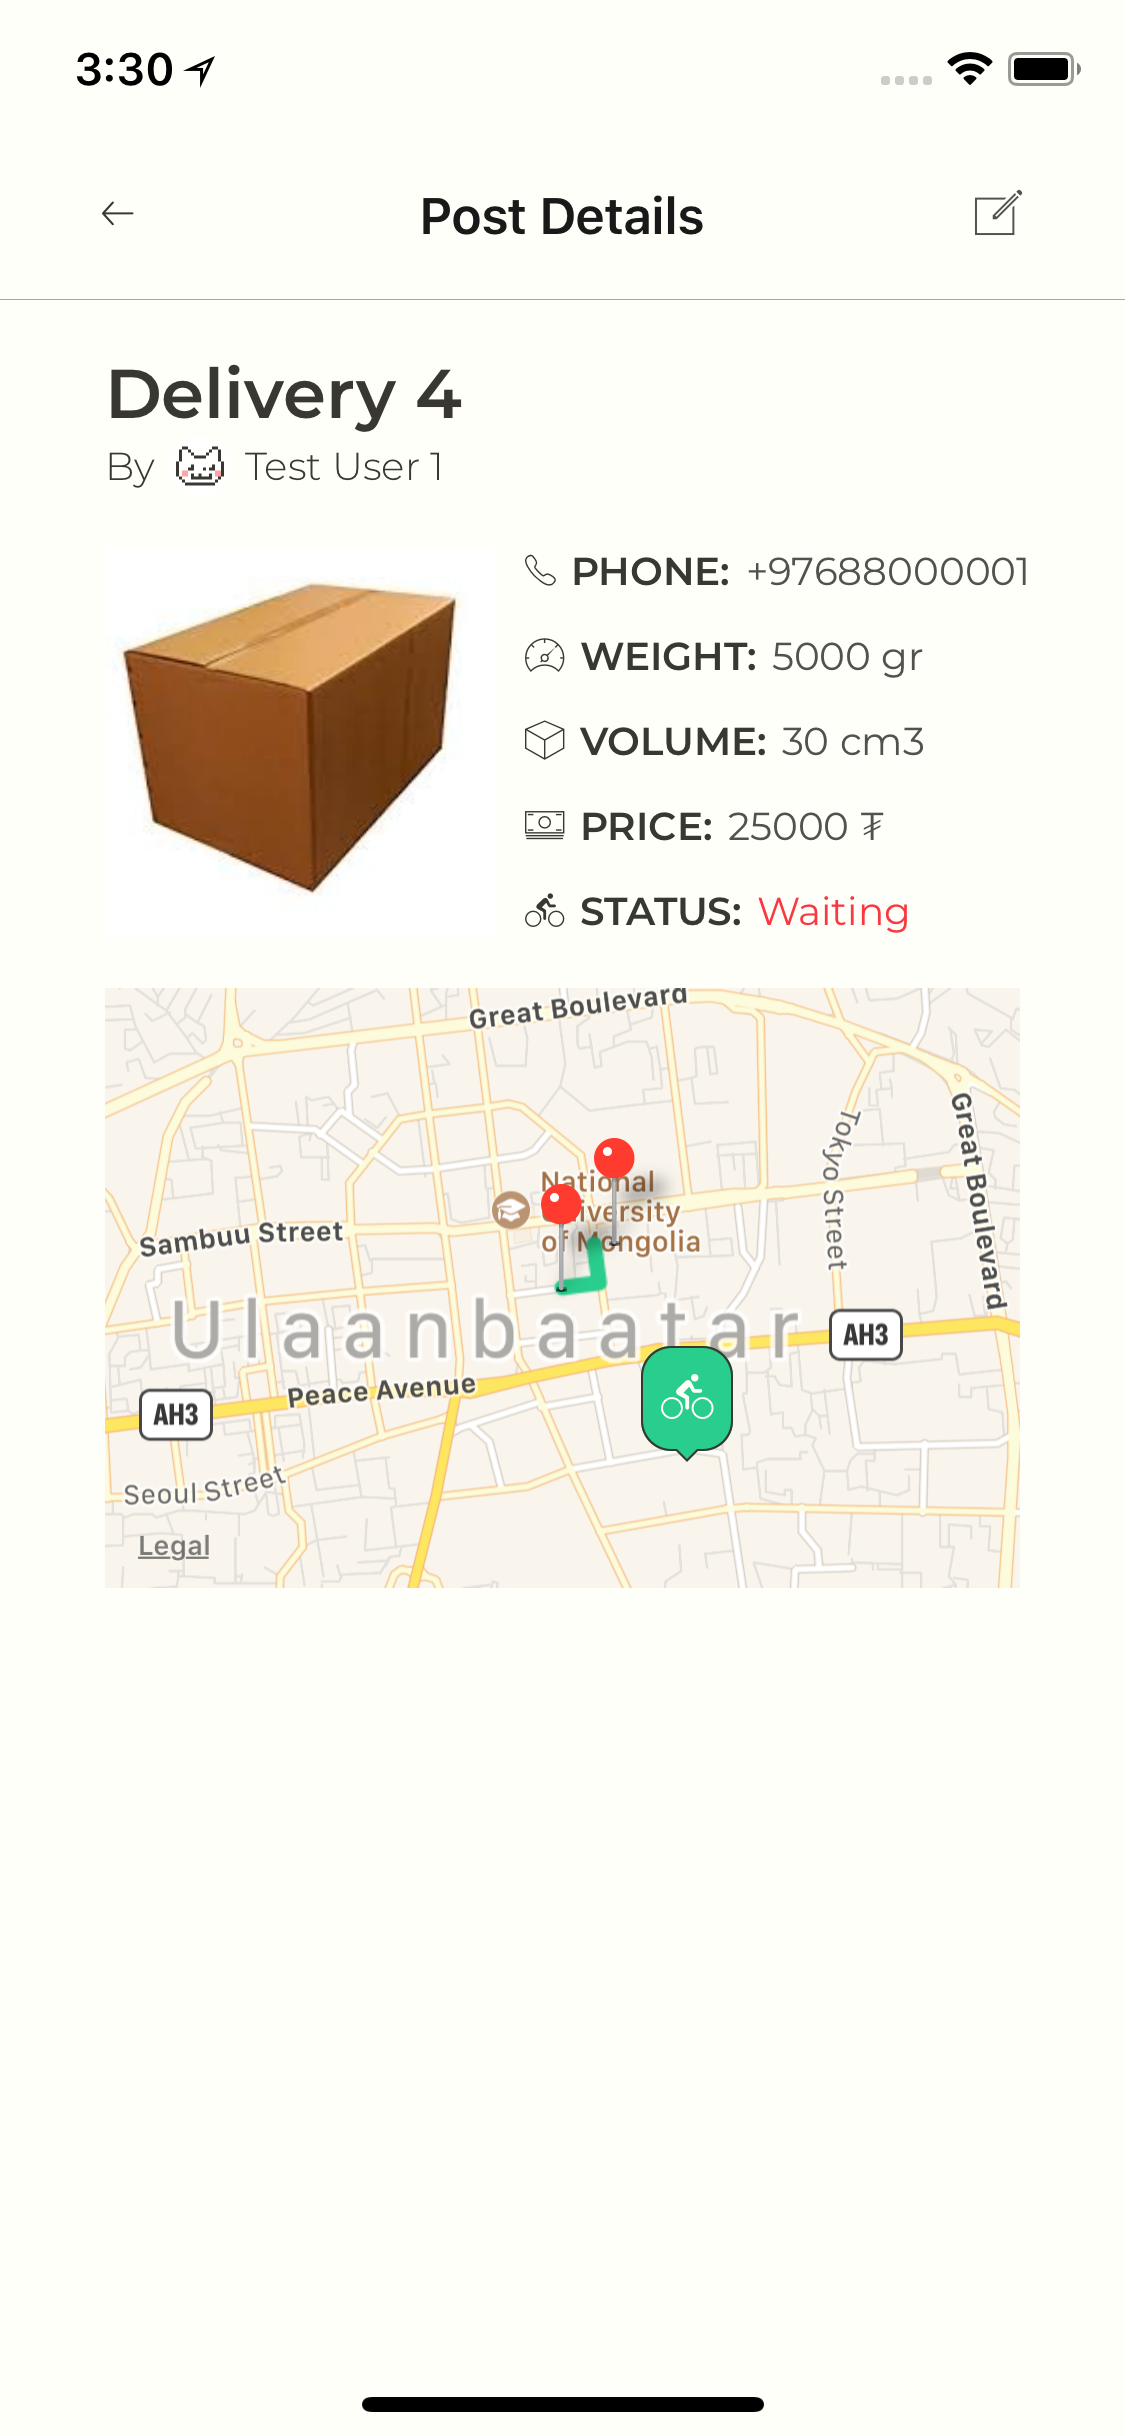
\includegraphics[width=.45\textwidth, frame]{Figures/interfaces/interface12.png}
    }
    \hfill
    \subcaptionbox{Хэрэглэгчийн үнэлгээнүүд}{
        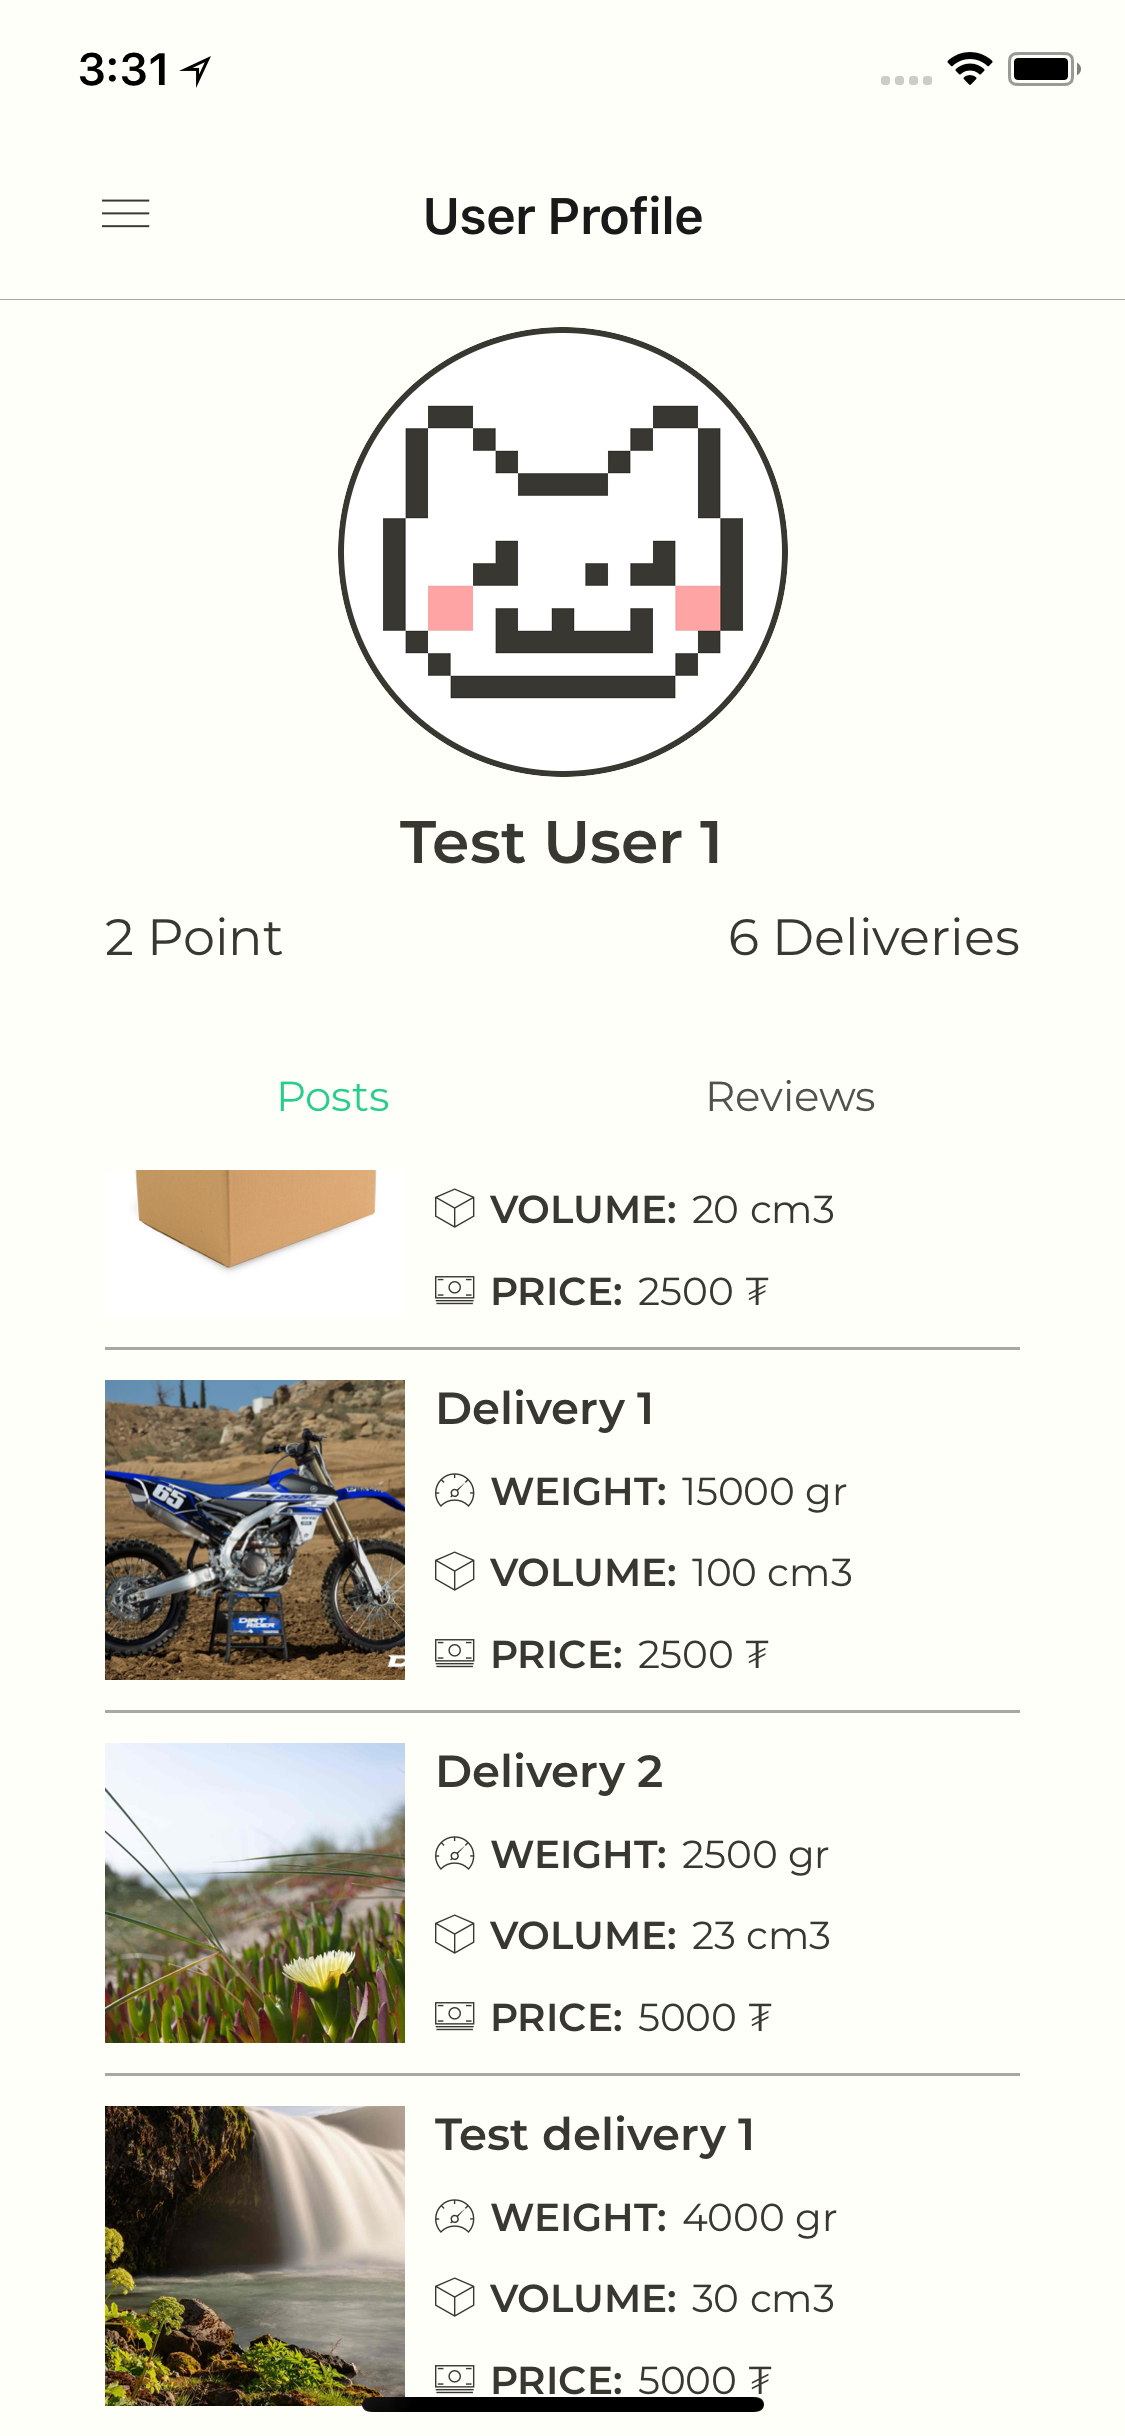
\includegraphics[width=.45\textwidth, frame]{Figures/interfaces/interface13.png}
    }
	\caption{Хэрэглэгчийн профайл дэлгэцийн интерфэйс}
\end{figure}

% \end{landscape} % Хуудсыг эргүүлэх

\section{Бүлгийн дүгнэлт}
Энэ бүлгийн хүрээнд уг төслийн ажлын зохиомжийн шатны бичиг баримтыг хийж гүйцэтгэсэн ба дараах зүйлсийг тодорхойлов:
\begin{itemize}[label={--}]
    \renewcommand\labelitemi{--}
    \item Өгөгдлийн ерөнхий схемийг гаргасан,
    \item Класс диаграмыг дүрсэлсэн,
    \item Дарааллын диаграмыг дүрсэлсэн,
    \item Хэрэглэгчийн интерфейсийг дүрсэлсэн болно.
\end{itemize}
